El hecho de que sea posible construir un sistema lineal que se asemeje significativamente a otro sistema, eventualmente no lineal, sugiere la viabilidad de emplear dicho sistema linealizado para abordar problemas de filtraje no lineal mediante el uso del Filtro de Kalman. 

En la literatura, ya existen diversas conexiones entre el Filtro de Kalman y el operador de Koopman. Por ejemplo, se ha explorado su utilización para la corrección de errores \cite{Jiang2022CorrectingFilters}, la estimación de modos de Koopman \cite{Liu2024EstimateFilter}, y la mejora de algoritmos como el Filtro de Kalman Extendido \cite{Ramadan2024ExtendedControl}. Además, algoritmos similares al que se propone en este capítulo han sido presentados y validados en diferentes aplicaciones, como se observa en \cite{Wang2022KoopmanSystem, Wang2023Innovation-saturatedOutliers, Netto2018RobustEstimation, Syed2021Koopman-basedXFEL, HuangData-DrivenFlight, Yang2025Data-DrivenPredictor}. 

Por otra parte, trabajos pioneros en la línea de observabilidad e identificación de sistemas, liderados por Surana y colaboradores, han proporcionado una base sólida en este campo, como se documenta en \cite{Surana2016KoopmanSystems, Surana2016LinearFramework}.

Por otro lado, hay enfoques que aplican la \textit{kernel Bayes Rule} a sistemas dinámicos y filtraje, donde se incluyen los trabajos de Song, Fukumizu y colaboradores \cite{Fukumizu2004DimensionalitySpaces, Fukumizu2013KernelKernels, Fukumizu2015NonparametricEmbedding, Song2009HilbertSystems, Song2013KernelModels}, lo que aparece de manera natural al demostrar la utilidad de los operadores para representar esperanzas condicionales.

Aunque el algoritmo propuesto en este capítulo no constituye una contribución original en términos de su estructura, sí lo es la justificación de su funcionamiento y convergencia bajo el supuesto de contar con un muestreo suficiente de puntos. En este contexto, se demuestra, en base a las cotas probadas anteriormente para la aproximación vía \textit{kernel} Dynamic Mode Decomposition, que un filtro subóptimo representado en dimensión finita converge al óptimo en dimensión infinita. 

El objetivo principal de este capítulo es demostrar que, bajo ciertas hipótesis, la tasa de convergencia del algoritmo es del orden de $N^{-1/2}$, lo que lo posiciona como un competidor viable frente a otros algoritmos de filtraje presentes en la literatura, tales como los filtros de partículas, discutidos previamente en la sección de preliminares.

Para ello, se propone primero descomponer el error del Filtro de Kalman aplicado a dos sistemas lineales, formulando este error en función de los datos provenientes de los sistemas. Este análisis, hasta la fecha de redacción de este trabajo, no se encuentra documentado en la literatura y, por lo tanto, constituye una contribución original de esta investigación.

Posteriormente, se construye el filtro propuesto, denominado \textit{Koopman Kalman Filter} (KKF), siguiendo una metodología análoga a la empleada en el Filtro de Kalman para sistemas lineales con mínimos cuadrados recursivos \cite{Kalman1960AProblems, Triantafyllopoulos2021BayesianBeyond}, y particularmente a como se formula en \cite{Gebhard2019} para la construcción de la denominada \textit{kernel Kalman Rule}.

Finalmente, utilizando los resultados obtenidos en el capítulo anterior junto con la descomposición del error, se demuestra la cota de error propuesta. El desempeño del filtro es evaluado en diferentes sistemas mediante una implementación en Python desarrollada específicamente para este trabajo.

Se muestran resultados numéricos del filtro en modelos epidemiológicos, tanto en problemas de filtraje con observaciones parciales como problemas de estimación de parámetros de estos modelos. El trabajo de Catalán Muñoz \cite{CatalanMunoz2022DesarrolloChile} fue una inspiración para este trabajo al aplicar Filtro de Kalman para estimación de parámetros de un modelo epidemiológico relevante para la realidad de Santiago de Chile. Cabe notar que Mezić et al. ya han aplicado técnicas relacionadas con operador de Koopman para modelos epidemiológicos \cite{Mezic2024ACases}, aunque nunca se habla de filtraje, dinámicas específicas ni estimación de parámetros. 

\section{Descomposición de error de Kalman}

El objetivo de esta sección es analizar el error que se genera entre dos reglas de Kalman, lo cual permitirá cuantificar la discrepancia entre una regla de Kalman aproximante y otra exacta, ambas definidas formalmente más adelante en esta misma sección. Para ello se asumirá que el horizonte de tiempo $T$ es finito, lo que evita tener que preocuparse por el comportamiento de las constantes para tiempos largos.

Para este propósito, se consideran dos sistemas dinámicos observados en un espacio de Hilbert con espacios de estados $E_x$ y de observaciones $E_y$, descritos por las siguientes ecuaciones:  
\begin{equation*}
	\begin{aligned}
		\mu_{i,k}  &= A_{i,k} \mu_{i,k-1} + \nu_{i,k}, \\
		y_{i,k} &= C_{i,k} \mu_{i,k} + \xi_{i,k},
	\end{aligned}
\end{equation*}
donde $A_{i,k} : E_x \to E_x$ y $C_{i,k}: E_x \to E_y$ son operadores lineales; $\nu_{i,k} \in E_x$ y $\xi_{i,k} \in E_y$ representan variables aleatorias con segundo momento finito y operadores de covarianza $\mathcal{Q}_{i,k}$ y $\mathcal{R}_{i,k}$, respectivamente. Todo esto se considera para $i \in \{1,2\}$ y $k \geq 1$.

Cada uno de estos sistemas tiene asociada una regla de Kalman, la cual está definida por las siguientes expresiones:  
\begin{equation*}
	\begin{aligned}
		\mathcal{P}_{i,k}^- &= A_{i,k}^* \mathcal{P}_{i,k-1}^+ A_{i,k} + \mathcal{Q}_{i,k}, \\
		\S_{i,k} &= C_{i,k} \mathcal{P}_{i,k}^- C_{i,k}^* + \mathcal{R}_{i,k}, \\
		\K_{i,k} &= \mathcal{P}_{i,k}^- C_{i,k} \S_{i,k}^{-1}, \\
		\mathcal{P}_{i,k}^+ &= (I - \K_{i,k} C_{i,k}) \mathcal{P}_{i,k}^-, \\
		\hat{\mu}_{i,k} &= A_{i,k} \hat{\mu}_{i,k-1} + \K_{i,k} (y_{i,k} - C_{i,k} \hat{\mu}_{i,k-1}),
	\end{aligned}
\end{equation*}
con $i \in \{1,2\}$ y $k \geq 1$. Aquí, $\mathcal{P}_{i,k}^-$ y $\mathcal{P}_{i,k}^+$ representan los operadores de covarianza del error a priori y a posteriori, respectivamente, mientras que $\K_{i,k}$ es el operador de ganancia de Kalman, todos ellos definidos en los espacios indicados. Estas reglas se inicializan como sigue:
\begin{equation*}
	\hat{\mu}_{i,0} = \mathbb{E}[\mu_{i,0}], \quad \mathcal{P}_{i,0} = \text{Cov}(\mu_{i,0}).
\end{equation*}

Con estas definiciones, se presenta un resultado clave que ilustra cómo la discrepancia en norma entre las reglas de Kalman puede descomponerse en función de las discrepancias en norma de los elementos asociados, junto con la influencia de las iteraciones previas.


\begin{teo}[Descomposición de error de Kalman]
	Sea $k \geq 1$. Si los operadores $\S_{i,k}$ son invertibles, entonces existen constantes $c_{k,j}^i$ con $j \in \{1, \dots, 7\}$, $i \in \{1, 2\}$, tales que se cumplen las siguientes desigualdades:
	\begin{equation*}
		\begin{aligned}
			\| \hat{\mu}_{1,k} - \hat{\mu}_{2,k} \| \leq & \, c_{1,k}^1 \| A_{1,k} - A_{2,k} \| + c_{2,k}^1 \| C_{1,k} - C_{2,k} \| \\ 
			&+ c_{3,k}^1 \| \mathcal{Q}_{1,k} - \mathcal{Q}_{2,k} \| + c_{4,k}^1 \| \mathcal{R}_{1,k} - \mathcal{R}_{2,k} \| \\
			&+ c_{5,k}^1 \| y_{1,k} - y_{2,k} \| + c_{6,k}^1 \| \hat{\mu}_{1,k-1} - \hat{\mu}_{2,k-1} \| \\
			&+ c_{7,k}^1 \| \mathcal{P}_{1,k-1}^+ - \mathcal{P}_{2,k-1}^+ \|,
		\end{aligned}
	\end{equation*}
	y
	\begin{equation*}
		\begin{aligned}
			\| \mathcal{P}_{1,k}^+ - \mathcal{P}_{2,k}^+ \| \leq & \, c_{1,k}^2 \| A_{1,k} - A_{2,k} \| + c_{2,k}^2 \| C_{1,k} - C_{2,k} \| \\ 
			&+ c_{3,k}^2 \| \mathcal{Q}_{1,k} - \mathcal{Q}_{2,k} \| + c_{4,k}^2 \| \mathcal{R}_{1,k} - \mathcal{R}_{2,k} \| \\
			&+ c_{5,k}^2 \| y_{1,k} - y_{2,k} \| + c_{6,k}^2 \| \hat{\mu}_{1,k-1} - \hat{\mu}_{2,k-1} \| \\
			&+ c_{7,k}^2 \| \mathcal{P}_{1,k-1}^+ - \mathcal{P}_{2,k-1}^+ \|.
		\end{aligned}
	\end{equation*}

	Aquí, las constantes $c_{k,j}^i$ son positivas y dependen de $k$ únicamente a través de las normas $\| A_{i,k} \|$, $\| C_{i,k} \|$, $\| \mathcal{Q}_{i,k} \|$, $\| \mathcal{R}_{i,k} \|$, $\| \S_{i,k}^{-1} \|$, $\| y_{i,k} \|$, $\| \hat{\mu}_{i,k-1} \|$ y $\| \mathcal{P}_{i,k-1}^+ \|$.
	\label{teo:error_kalman}
\end{teo}

\begin{proof}
Se observa que  
\begin{equation*}
	\begin{aligned}
		&	\| \hat \mu_{1,k} - \hat \mu_{2,k} \|_{E_x}  \\
		\leq & \, \| A_{1,k} \mu_{1,k-1}  - A_{2,k} \mu_{2,k-1} \|  \\
		& + \|  \K_{1,k} (y_{1,k} - C_{1,k} \hat\mu_{1,k-1}) -  \K_{2,k} (y_{2,k} - C_{2,k} \hat\mu_{2,k-1})  \|.
	\end{aligned}
\end{equation*}
El primer término, denominado \textit{error de predicción}, satisface la siguiente desigualdad:
\begin{equation*}
	\begin{aligned}
		& \| A_{1,k} \mu_{1,k-1}  - A_{2,k} \mu_{2,k-1} \|  \\
		& \leq \| A_{1,k} \mu_{1,k-1}  - A_{1,k} \mu_{2,k-1} \| + \| A_{1,k} \mu_{2,k-1}  - A_{2,k} \mu_{2,k-1} \| \\
		& \leq \| A_{1,k} \| \| \mu_{1,k-1}  - \mu_{2,k-1} \| +  \| \mu_{2,k-1} \| \| A_{1,k} - A_{2,k} \|.
	\end{aligned}
\end{equation*}
Por otro lado, el segundo término, denominado \textit{error de actualización}, cumple:
\begingroup
\allowdisplaybreaks
\begin{align*}
    & \|  \K_{1,k} (y_{1,k} - C_{1,k} \hat\mu_{1,k-1}) -  \K_{2,k} (y_{2,k} - C_{2,k} \hat\mu_{2,k-1})  \| \\
		& \leq  \| \K_{1,k} y_{1,k} -  \K_{2,k} y_{2,k}  \| + \| \K_{1,k} C_{1,k} \hat\mu_{1,k-1} - \K_{2,k} C_{2,k} \hat\mu_{2,k-1}  \| \\
		& \leq \| \K_{1,k} y_{1,k} -  \K_{1,k} y_{2,k}  \| + \| \K_{1,k} y_{2,k} -  \K_{2,k} y_{2,k}  \| \\
		& \quad + \| \K_{1,k} C_{1,k} \hat\mu_{1,k-1} - \K_{1,k} C_{2,k} \hat\mu_{2,k-1}  \| + \| \K_{1,k} C_{2,k} \hat\mu_{2,k-1} - \K_{2,k} C_{2,k} \hat\mu_{2,k-1}  \| \\
		& \leq \| \K_{1,k} \| \|  y_{1,k} - y_{2,k}  \| + \| y_{2,k} \| \| \K_{1,k}  -  \K_{2,k}  \| \\
		& \quad + \| \K_{1,k} \| \|  C_{1,k} \hat\mu_{1,k-1} - C_{2,k} \hat\mu_{2,k-1}  \| + \| C_{2,k} \hat\mu_{2,k-1} \| \| \K_{1,k}  - \K_{2,k} \| \\
		& \leq \| \K_{1,k} \| \|  y_{1,k} - y_{2,k}  \| + \| y_{2,k} \| \| \K_{1,k}  -  \K_{2,k}  \| \\
		& \quad + \| \K_{1,k} \| \left ( \|  C_{1,k} \hat\mu_{1,k-1} - C_{1,k} \hat\mu_{2,k-1}  \| + \|  C_{1,k} \hat\mu_{2,k-1} - C_{2,k} \hat\mu_{2,k-1}  \| \right ) \\
		& \quad + \| C_{2,k} \hat\mu_{2,k-1} \| \| \K_{1,k}  - \K_{2,k} \| \\
		& \leq \| \K_{1,k} \| \|  y_{1,k} - y_{2,k}  \| + \| y_{2,k} \| \| \K_{1,k}  -  \K_{2,k}  \| \\
		& \quad + \| \K_{1,k} \| \left ( \| C_{1,k}  \| \|  \hat\mu_{1,k-1} - \hat\mu_{2,k-1}  \| + \| \hat\mu_{2,k-1}  \| \| C_{1,k} - C_{2,k}  \| \right ) \\
		& \quad + \| C_{2,k} \hat\mu_{2,k-1} \| \| \K_{1,k}  - \K_{2,k} \|.
\end{align*}
\endgroup

En virtud de lo anterior, se debe analizar la diferencia en norma de los operadores de ganancia:
\begin{equation*}
	\begin{aligned}
		& \| \K_{1,k}  - \K_{2,k} \| \\
		& \leq \| \mathcal{P}_{1,k}^- C_{1,k}\S_{1,k}^{-1} -  \mathcal{P}_{2,k}^- C_{2,k} \S_{2,k}^{-1} \| \\
		& \leq \| \mathcal{P}_{1,k}^- C_{1,k}\S_{1,k}^{-1} - \mathcal{P}_{2,k}^- C_{1,k}\S_{1,k}^{-1} \| + \| \mathcal{P}_{2,k}^- C_{1,k}\S_{1,k}^{-1} - \mathcal{P}_{2,k}^- C_{2,k}\S_{2,k}^{-1} \| \\
		& \leq \| C_{1,k}\S_{1,k}^{-1} \| \| \mathcal{P}_{1,k}^- - \mathcal{P}_{2,k}^-\| + \| \mathcal{P}_{2,k}^- \| \|  C_{1,k}\S_{1,k}^{-1} -  C_{2,k}\S_{2,k}^{-1}\| \\
		& \leq \| C_{1,k}\S_{1,k}^{-1} \| \| \mathcal{P}_{1,k}^- - \mathcal{P}_{2,k}^-\| \\
		& \quad + \| \mathcal{P}_{2,k}^- \| ( \|  C_{1,k}\S_{1,k}^{-1} -  C_{1,k}\S_{2,k}^{-1}\| + \|  C_{1,k}\S_{2,k}^{-1} -  C_{2,k}\S_{2,k}^{-1}\|) \\
		& \quad + \| \mathcal{P}_{2,k}^- \| ( \|  C_{1,k} \| \| \S_{1,k}^{-1} -  \S_{2,k}^{-1}\| + \| \S_{2,k}^{-1} \| \| C_{1,k} -  C_{2,k}\|).
	\end{aligned}
\end{equation*}
En donde
\begin{equation*}
	\| \mathcal{P}_{i,k}^- \|  \leq \| A_{i,k} \|^2 \| \mathcal{P}_{i,k-1}^+\| + \| \mathcal{Q}_{i,k}\|, \quad i \in \{ 1, 2 \}.
\end{equation*}

Primero, para las diferencias en norma de los operadores de covarianza de error a priori se tiene:
\begin{equation*}
	\begin{aligned}
		& \| \mathcal{P}_{1,k}^- - \mathcal{P}_{2,k}^-\| \\
		& = \| A_{1,k}^* \mathcal{P}_{1,k-1}^+ A_{1,k} + \mathcal{Q}_{1,k} - A_{2,k}^* \mathcal{P}_{2,k-1}^+ A_{2,k} + \mathcal{Q}_{2,k}  \| \\
		& \leq \|A_{1,k}^* \mathcal{P}_{1,k-1}^+ A_{1,k} - A_{2,k}^* \mathcal{P}_{2,k}^+ A_{2,k} \| + \| \mathcal{Q}_{1,k} - \mathcal{Q}_{2,k}  \| \\
		& \leq \|A_{1,k}^* \mathcal{P}_{1,k-1}^+ A_{1,k} - A_{1,k}^* \mathcal{P}_{2,k-1}^+ A_{2,k} \| +  \|A_{1,k}^* \mathcal{P}_{2,k-1}^+ A_{2,k} - A_{2,k}^* \mathcal{P}_{2,k-1}^+ A_{2,k} \| \\ 
		& \quad + \| \mathcal{Q}_{1,k} - \mathcal{Q}_{2,k}  \| \\
		& \leq \|A_{1,k}^* \| \| \mathcal{P}_{1,k-1}^+ A_{1,k} - \mathcal{P}_{2,k-1}^+ A_{2,k} \| + \| \mathcal{P}_{2,k-1}^+ A_{2,k}  \| \|A_{1,k}^* - A_{2,k}^* \| \\ 
		& \quad + \| \mathcal{Q}_{1,k} - \mathcal{Q}_{2,k}  \| \\
		& \leq \|A_{1,k} \| \| \mathcal{P}_{1,k-1}^+ A_{1,k} - \mathcal{P}_{2,k-1}^+ A_{2,k} \| + \| \mathcal{P}_{2,k-1}^+ A_{2,k}  \| \|A_{1,k} - A_{2,k} \| \\ 
		& \quad + \| \mathcal{Q}_{1,k} - \mathcal{Q}_{2,k}  \| \\
		& \leq \|A_{1,k} \| (\| \mathcal{P}_{1,k}^+ A_{1,k} - \mathcal{P}_{1,k-1}^+ A_{2,k} \| + \| \mathcal{P}_{1,k-1}^+ A_{2,k} - \mathcal{P}_{2,k-1}^+ A_{2,k} \| ) \\
		& \quad + \| \mathcal{P}_{2,k-1}^+ \| \| A_{2,k}  \| \|A_{1,k} - A_{2,k} \| \\ 
		& \quad + \| \mathcal{Q}_{1,k} - \mathcal{Q}_{2,k}  \| \\
		& \leq \|A_{1,k} \| ( \| \mathcal{P}_{1,k-1}^+ \| \|  A_{1,k} - A_{2,k} \| + \| A_{2,k} \| \| \mathcal{P}_{1,k-1}^+  - \mathcal{P}_{2,k-1}^+  \| ) \\
		& \quad + \| \mathcal{P}_{2,k-1}^+ \| \| A_{2,k}  \| \|A_{1,k} - A_{2,k} \| \\ 
		& \quad + \| \mathcal{Q}_{1,k} - \mathcal{Q}_{2,k}  \|.
	\end{aligned}
\end{equation*}

Se analizará finalmente el término $\| \S_{1,k}^{-1} -  \S_{2,k}^{-1}\|$. Para ello, se observa que
\begin{equation*}
	\S_{1,k}^{-1} -  \S_{2,k}^{-1} = \S_{2,k}^{-1} (\S_{2,k} - \S_{1,k}) \S_{1,k}^{-1}.
\end{equation*}
A partir de esta expresión, se tiene que
\begin{equation*}
	\begin{aligned}
		\| \S_{1,k}^{-1} -  \S_{2,k}^{-1} \| & \leq  \| \S_{2,k}^{-1} (\S_{2,k} - \S_{1,k}) \S_{1,k}^{-1} \| \\
		& \leq \| \S_{1,k}^{-1} \| \|  \S_{2,k}^{-1} \| \| \S_{2,k} - \S_{1,k}\| \\
		& \leq  \| \S_{1,k}^{-1} \| \|  \S_{2,k}^{-1} \|  \| C_{1,k} \mathcal{P}_{1,k}^- C_{1,k}^* + \mathcal{R}_{1,k} - C_{2,k} \mathcal{P}_{2,k}^- C_{2,k}^* + \mathcal{R}_{2,k} \|.
	\end{aligned}
\end{equation*}
En este contexto, y de manera análoga a lo previamente demostrado, se obtiene la siguiente estimación para la expresión anterior:
\begin{equation*}
	\begin{aligned}
		\| C_{1,k} \mathcal{P}_{1,k}^- C_{1,k}^* + \mathcal{R}_{1,k} - C_{2,k} \mathcal{P}_{2,k}^- C_{2,k}^* + \mathcal{R}_{2,k} \| \\
		& \leq \|C_{1,k-1} \|  \| \mathcal{P}_{1,k-1}^+ \| \|  C_{1,k} - C_{2,k} \|  \\
            & \quad + \|C_{1,k-1} \|  \| C_{2,k} \| \| \mathcal{P}_{1,k-1}^+  - \mathcal{P}_{2,k-1}^+  \| \\
		& \quad + \| \mathcal{P}_{2,k-1}^+ \| \| C_{2,k}  \| \|C_{1,k} - C_{2,k} \| \\
		& \quad+ \| \mathcal{R}_{1,k} - \mathcal{R}_{2,k}  \|.
	\end{aligned}
\end{equation*}

\end{proof}

Con lo anterior, se concluye que, para una iteración $k$, el error depende tanto del error en la condición para la estimación del estado como del operador de covarianza del error a posteriori.

\section{Koopman Kalman Filter}

En esta sección se presenta la deducción del algoritmo de filtraje solo utilizando la teoría de RKHS junto con el operador de Koopman de manera meticulosa. Primero se deduce una dinámica del \textit{embedding}, y sus observaciones asociadas.

\begin{prop}
    El \textit{embedding} de $\{\mathbf{x}_k\}_{k=0}^T$ en $\H_\X$ satisface
    \begin{align*}
        \Phi_\X (\mathbf{x}_{k+1}) &= C_{X^+|X} \Phi_\X (\mathbf{x}_k) + \zeta_k \\
        \mathbf{y}_k &= C_{Y|X} \Phi_\X (\mathbf{x}_k) + \nu_k,
    \end{align*}
    donde $\zeta_k$ y $\nu_k$ son realizaciones de variables aleatorias a valores en $\H_\X$ y $\R^p$, respectivamente, ambas con media nula y segundo momento finito, con operador de covarianza $\mathcal{Q}_k : \H_\X \to \H_\X$ y matriz de covarianza $\mathcal{R}_k \in \R^{p \times p}$ semidefinida positiva, respectivamente. Si además, $\mathbf{g}$ cumple que
    \begin{equation}
    \label{eq:condi_g}
        \E[\| (\mathbf{g}(\mathbf{x}, \cdot) - \E[\mathbf{g}(\mathbf{x}, \cdot)])^\top v \|] = 0 \iff v = 0
    \end{equation}
    entonces $\mathcal{R}_k \in \R^{p \times p}$ es definida positiva.
\end{prop}

\begin{proof}
    Primero para la dinámica
    \begin{equation*}
	\begin{aligned}
		\Phi_\X (\mathbf{x}_{k+1}) &= \Phi_\X (\mathbf{f}(\mathbf{x}_k, \mathbf{w}_k)) \\
        &= \E[\Phi_\X (X^+) | X = \mathbf{x}_k] + \Phi_\X (\mathbf{f}(\mathbf{x}_k, \mathbf{w}_k)) - \E[\Phi_\X (X^+) | X = \mathbf{x}_k]\\
        &= C_{X^+|X} \Phi_\X (\mathbf{x}_k) + \zeta_k
	\end{aligned}
\end{equation*}
donde 
\begin{equation*}
    \zeta_k = \Phi_\X (\mathbf{f}(\mathbf{x}_k, \mathbf{w}_k)) - \E[\Phi_\X (X^+) | X = \mathbf{x}_k]
\end{equation*}
es una variable aleatoria infinita dimensional cuyo operador de covarianza está acotado y se denota por 
\[
\mathcal{Q}_k := \int_\X \Phi_\X (x) \otimes \Phi_\X(x) d \rho_f (\mathbf{x}_k,x). 
\]
Además, esta variable aleatoria tiene media nula, esto ya que
\begin{equation*}
    \mathbf{f}(\mathbf{x}_k, \mathbf{w}_k) \sim X^+ | X = \mathbf{x}_k,
\end{equation*}
con lo que
\begin{equation*}
    \begin{aligned}
         \E[\zeta_k] &= \E[\Phi_\X (\mathbf{f}(\mathbf{x}_k, \mathbf{w}_k))] - \E[\E[\Phi_\X (X^+) | X = \mathbf{x}_k]] \\
         &= \E[\E[\Phi_\X (X^+) | X = \mathbf{x}_k]] - \E[\E[\Phi_\X (X^+) | X = \mathbf{x}_k]] \\
         &= 0.
    \end{aligned}
\end{equation*}
De manera análoga, para el \textit{embedding} de la observación se tiene
\begin{equation*}
	\begin{aligned}
		\Phi_\Y (\mathbf{y}_{k}) &= \Phi_\Y (\mathbf{g}(\mathbf{x}_k, \mathbf{v}_k)) \\
        &= \E[\Phi_\Y (Y) | X = \mathbf{x}_k] + \Phi_\Y (\mathbf{g}(\mathbf{x}_k, \mathbf{v}_k)) - \E[\Phi_\Y (Y) | X = \mathbf{x}_k]\\
        &= C_{Y|X} \Phi_\X (\mathbf{x}_k) + \nu_k
	\end{aligned}
\end{equation*}
donde $\nu_k$ es una variable aleatoria infinita dimensional cuyo operador de covarianza está acotado, denotado por
\[
\mathcal{R}_k := \E[ (\mathbf{g}(\mathbf{x}, \cdot) - \E[\mathbf{g}(\mathbf{x}, \cdot)])^\top (\mathbf{g}(\mathbf{x}, \cdot) - \E[\mathbf{g}(\mathbf{x}, \cdot)]) ],
\]
que es semidefinida positiva ya que
\[
v^\top \E[ (\mathbf{g}(\mathbf{x}, \cdot) - \E[\mathbf{g}(\mathbf{x}, \cdot)])^\top (\mathbf{g}(\mathbf{x}, \cdot) - \E[\mathbf{g}(\mathbf{x}, \cdot)]) ] v = \E[\| (\mathbf{g}(\mathbf{x}, \cdot) - \E[\mathbf{g}(\mathbf{x}, \cdot)])^\top v \|^2] \geq 0,
\]
y si cumple \ref{eq:condi_g}, se cumple $\mathcal{R}_k $ es definida positiva. Y está centrada ya que
\begin{equation*}
    \mathbf{g}(\mathbf{x}_k, \mathbf{v}_k) \sim Y | X = \mathbf{x}_k
\end{equation*}
con lo que
\begin{equation*}
    \begin{aligned}
         \E[\nu_k] &= \E[\Phi_\Y (\mathbf{g}(\mathbf{x}_k, \mathbf{v}_k))] - \E[\E[\Phi_\Y (Y) | X = \mathbf{x}_k]] \\
         &= \E[\E[\Phi_\Y (Y) | X = \mathbf{x}_k]] - \E[\E[\Phi_\Y (Y) | X = \mathbf{x}_k]] \\
         &= 0.
    \end{aligned}
\end{equation*}
\end{proof}

\begin{obs}
    En lo que sigue se supondrá que se cumple \ref{eq:condi_g}, lo que hará que se satisfaga la hipótesis del teorema \ref{teo:error_kalman} sobre la invertibilidad de los $\mathcal{S}_k$ al ser suma de una matriz simétrica semidefinida positiva y una matriz simétrica definida positiva, argumento que también se verá en la deducción del operador de ganancia de Kalman. 
    
    Un ejemplo en donde esto se cumple es cuando $\mathbf{g}$ es aditiva y el ruido tiene matriz de covarianza definida positiva, esto es, si
    \[
    \mathbf{g}(\mathbf{x}, \mathbf{v}) = \Tilde{\mathbf{g}}(\mathbf{x}) + \mathbf{v}
    \]
    entonces
    \[
    \E[\mathbf{g}(\mathbf{x, \cdot)}] = \Tilde{\mathbf{g}}(\mathbf{x}),
    \]
    así
    $\mathcal{R}_k = \E[\mathbf{v_k} \mathbf{v_k}^\top]$, que es definida positiva.
\end{obs}

Siguiendo un procedimiento similar al utilizado en \cite{Gebhard2019}, se define
\begin{equation*}
	\hat{\mu}_k = \mathbb{E} [\Phi_\X (\mathbf{x}_k) | \mathbf{y}_{1:k}], \quad \mathcal{P}_{k} = \text{Cov}(\Phi_\X(\mathbf{x}_k) - \hat{\mu}_k)
\end{equation*}
con inicialización dada por
\begin{equation*}
	\hat{\mu}_0 = \hat{\mu}_0^- = \mathbb{E} [\Phi_\X (\mathbf{x}_0)], \quad \mathcal{P}_{0} = \text{Cov}(\Phi_\X (\mathbf{x}_0) - \hat{\mu}_0).
\end{equation*}
Se define también una forma para la predicción
\begin{equation*}
	\hat{\mu}_{k+1}^- = \mathbb{E} [\Phi_\X (\mathbf{x}_{k+1}) | \mathbf{y}_{1:k}], \quad \mathcal{P}_{k+1}^- = \text{Cov}(\Phi_\X (\mathbf{x}_{k+1}) - \hat{\mu}_{k+1}^-),
\end{equation*}
con lo que se entrega una forma más cerrada e iterativa para estos elementos.

\begin{prop}[Sobre la predicción]
    $\hat{\mu}_{k+1}^- $ y $\mathcal{P}_{k+1}^-$ satisfacen
    \[
    \hat{\mu}_{k+1}^- = C_{X^+|X} \hat{\mu}_k, \quad \mathcal{P}_{k+1}^- = C_{X^+|X} \mathcal{P}_k (C_{X^+|X})^* + \mathcal{Q}_{k+1}
    \]
\end{prop}

\begin{proof}
    Lo primero es directo de la \textit{kernel} Bayes Rule \cite{Fukumizu2013KernelKernels}, es decir
\begin{equation*}
	\hat{\mu}_{k+1}^- = \mathbb{E} [\Phi_\X (\mathbf{x}_{k+1}) | \mathbf{y}_{1:k}] = C_{X^+|X} \mathbb{E} [\Phi_\X (\mathbf{x}_{k}) | \mathbf{y}_{1:k}] = C_{X^+|X} \hat{\mu}_k.
\end{equation*}
A partir de esto, y utilizando la independencia de $\zeta_k$ con respecto a $\Phi_\X (\mathbf{x}_k)$, se obtiene
\begin{equation*}
	\begin{aligned}
		\mathcal{P}_{k+1}^- &= \text{Cov}(\Phi_\X (\mathbf{x}_{k+1}) - \hat{\mu}_{k+1}^-)  \\
		&= \text{Cov}(C_{X^+|X}\Phi_\X (\mathbf{x}_{k}) + \zeta_{k+1} - C_{X^+|X}\hat{\mu}_{k}) \\
		&= C_{X^+|X} \text{Cov} (\Phi_\X (\mathbf{x}_{k}) - \hat{\mu}_{k})C_{X^+|X}^* + \text{Cov}(\zeta_{k+1}) \\
		&= C_{X^+|X} \mathcal{P}_k (C_{X^+|X})^* + \mathcal{Q}_{k+1}
	\end{aligned}
\end{equation*}
\end{proof}

Posteriormente, se debe proyectar sobre las observaciones para obtener la estimación a posteriori, es decir,
\begin{equation*}
	\hat{\mu}_{k+1}^- = \mathbb{E} [\Phi_\X (\mathbf{x}_{k+1}) | \mathbf{y}_{1:k}] \quad \text{se actualiza a} \quad \hat{\mu}_{k+1} = \mathbb{E} [\Phi_\X (\mathbf{x}_{k+1}) | \mathbf{y}_{1:k+1}].
\end{equation*}

Por lo que se debe agregar un factor de proyección, que indique la dirección a proyectar, por lo que propone un operador $\K_k : \mathbb{R}^p \to \mathcal{H}_\X$, denominado el operador de ganancia de Kalman, tal que
\begin{equation*}
	\hat{\mu}_{k+1} = \hat{\mu}_{k+1}^- + \K_{k+1} (\mathbf{y}_{k+1} - C_{Y|X} \hat{\mu}_{k+1}^-).
\end{equation*}
En Gebhardt et al. \cite{Gebhard2019} se deduce que $\hat{\mu}_k$ es un estimador insesgado de $\mu_k$, para todo $k$ y además una expresión para el operador de ganancia, que se deja a continuación por completitud de la deducción del filtro, en donde se ha ajustado la notación a lo presentado anteriormente.

\begin{prop}[Sobre la actualización, Adaptación de Gebhardt et al. \cite{Gebhard2019}]
\label{prop:unbias_kalman_operator}
    El estimador $\hat{\mu}_k$ es insesgado para $\mu_k$, para todo $k$ y el operador de ganancia de Kalman $\K_k: \R^p \to \H_\X$ viene dado por
    \begin{equation*}
        \mathcal{K}_k = \mathcal{P}^-_{k}C_{Y|X}^*(C_{Y|X}\mathcal{P}^-_{k}C_{Y|X}^* + \mathcal{R}_k)^{-1}.
    \end{equation*}
    Además, el operador de covarianza de error a posteriori viene dado por
    \begin{equation*}
    \mathcal{P}_k = (I - \K_k C_{Y|X})\mathcal{P}^-_{k}.
\end{equation*}
\end{prop}
\begin{proof}
    Denotando $\varepsilon_k^- = \hat{\mu}_k^- - \mu_k \in \H_\X$ el error a priori y $\varepsilon_k^+ = \hat{\mu}_k - \mu_k \in \H_\X$ el error a posteriori, se tiene lo siguiente
    \begin{align*}
    \varepsilon_k^+ &= \hat{\mu}_k - \mu_k \\
                &=\hat{\mu}_{k}^- + \K_{k} (\mathbf{y}_{k} - C_{Y|X} \hat{\mu}_{k}^-) - \mu_k \\
                &= \varepsilon_k^- +  \K_{k} \mathbf{y}_{k} - \K_k C_{Y|X} \hat{\mu}_{k}^- \\
                &= \varepsilon_k^- +  \K_{k} \mathbf{y}_{k} - \K_k C_{Y|X} \hat{\mu}_{k}^- + \K_k C_{Y|X} \mu_k - \K_k C_{Y|X} \mu_k\\
                &= \varepsilon_k^- + \K_k C_{Y|X} (-\hat{\mu}_{k}^- + \mu_k) + \K_{k} \mathbf{y}_{k} - \K_k C_{Y|X} \mu_k\\
                &= \varepsilon_k^- - \K_k C_{Y|X}  \varepsilon_k^- + \K_{k} \mathbf{y}_{k} - \K_k C_{Y|X} \mu_k\\
                &= ( I - \K_k C_{Y|X} ) \varepsilon_k^- + \K_{k} (\mathbf{y}_{k} - C_{Y|X} \mu_k)\\
                &= ( I - \K_k C_{Y|X} ) \varepsilon_k^- + \K_{k} \nu_k
\end{align*}

Primero se probará que $\E[\varepsilon_k^-] = 0$, esto por inducción. En primer lugar, para $k=0$ se tiene por construcción, con lo que el caso el caso base queda probado. Suponiendo que se cumple para $k \in \N$, se propone probarlo para $k+1$. Notando que 
\begin{equation*}
    \varepsilon_{k+1}^- = \hat{\mu}_{k+1}^- - \mu_{k+1} = C_{X^+|X} \hat{\mu}_k - C_{X^+|X} \mu_k - \zeta_k,
\end{equation*}
se tiene que
\begin{equation*}
    \E[\varepsilon_{k+1}^-] = C_{X^+|X} \E [\hat{\mu}_k] - \E[\zeta_k] = C_{X^+|X} \E[\varepsilon^+_k],
\end{equation*}
ya que las variables aleatorias $\zeta_k$ son centradas. Con ello
\begin{equation*}
    \E[\varepsilon^+_k] = ( I - \K_k C_{Y|X} ) \E[\varepsilon_k^-] + \K_{k} \E[\nu_k] = 0,
\end{equation*}
ya los $\nu_k$ son centrados y por la hipótesis de inducción $\E[\varepsilon_k^-] = 0$. Luego por principio de inducción queda probado que $\E[\varepsilon_k^-] = 0$, para todo $k$.  Haciendo la misma manipulación de antes, se prueba que $\E[\varepsilon^+_k] = 0$, para todo $k$, con lo que el estimado $\hat{\mu}_k$ es insesgado para $\mu_k$.

Ahora para el operador de ganancia se debe recordar que en el problema de filtraje se busca minimizar la pérdida cuadrática esperada asociada a la estimación de la trayectoria, la que viene dada por
\begin{equation*}
    \E[(\hat{\mu}_{k} - \mu_{k})^* (\hat{\mu}_{k} - \mu_{k}) ] = \E [ (\varepsilon_k^+)^* \varepsilon_k^+ ].
\end{equation*}
Dado que el estimador es insesgado, esto se puede reformular como la minimización de la traza de la covarianza de error a posteriori $\mathcal{P}_k$, es decir
\begin{align*}
\min_{\K_k} \mathbb{E}[(\varepsilon_k^+)^* \varepsilon_k^+] &= \min_{\K_k} \text{Tr} \mathbb{E}[\varepsilon_k^+(\varepsilon_k^+)^*] \\
&= \min_{\K_k} \text{Tr} \mathcal{P}_{k}.
\end{align*}
Sustituyendo la expresión para el error a posteriori se tiene que
\begin{align*}
\mathcal{P}_k &= \mathbb{E}[\varepsilon^+_k(\varepsilon^+_k)^*] \\
&= \mathbb{E}[((I - \K_k C_{Y|X})\varepsilon^-_k - \K_k \nu_k)((I - \K_k C_{Y|X})\varepsilon^-_k - \K_k \nu_k)^*] \\
&= (I - \K_k C_{Y|X})\mathbb{E}[\varepsilon^-_k(\varepsilon^-_k)^*](I - \K_k C_{Y|X})^* 
- \K_k\mathbb{E}[\nu_k(\varepsilon^-_k)^*](I - \K_k C_{Y|X})^* \\
&\quad - (I - \K_k C_{Y|X})\mathbb{E}[\varepsilon^-_k\nu_k^*]\K_k^* + \K_k\mathbb{E}[\nu_k\nu_k^*]\K_k^*.
\end{align*}
Dado que se asume que el ruido del operador de observación es independiente del error de estimación y dado que se asumió que la estimación a priori tiene media cero, se obtiene
\begin{equation*}
\mathbb{E}[\nu_k(\varepsilon^-_k)^*] = \mathbb{E}[\nu_k]\mathbb{E}[(\varepsilon^-_k)^*] = \mathbb{E}[(\varepsilon^-_k)^*]\mathbb{E}[\nu_k] = \mathbb{E}[\varepsilon^-_k\nu_k^*] = 0.
\end{equation*}

Con esta perspectiva, el operador de covarianza posterior puede reformularse como
\begin{equation*}
\mathcal{P}_k = (I - \K_k C_{Y|X})\mathcal{P}^-_{k}(I - \K_k C_{Y|X})^* + \K_k \mathcal{R}_k \K_k^*,
\end{equation*}
donde $\mathcal{R}_k = \mathbb{E}[\nu_k\nu_k^*]$ es la covarianza del ruido asociado a la observación. Tomando la derivada de la traza del operador de covarianza con respecto del operador de ganancia e igualándola a cero se obtiene
\begin{align*}
2(I - \K_k C_{Y|X})\mathcal{P}^-_{k}(-C_{Y|X}^*) + 2\K_k \mathcal{R}_k &= 0,
\end{align*}
que es equivalente a 
\begin{equation}
    -(I - \K_k C_{Y|X})\mathcal{P}^-_{k}C_{Y|X}^* + \K_k \mathcal{R}_k = 0.
    \label{eq:kalman_gain_rel}
\end{equation}

Con esto
\begin{align*}
\K_k C_{Y|X}\mathcal{P}^-_{k}C_{Y|X}^* + \K_k \mathcal{R}_k &= \K^-_{k}C_{Y|X}^*, \\
\K_k(C_{Y|X}\mathcal{P}^-_{k}C_{Y|X}^* + \mathcal{R}_k) &= \mathcal{P}^-_{k}C_{Y|X}^* .
\end{align*}
Aquí la decisión $\H_\Y = (\R^p)^*$ cobra sentido, ya que entonces, dado que $\mathcal{R}_k$ es una matriz simétrica definida positiva, es invertible, como $C_{Y|X}\mathcal{P}^-_{k}C_{Y|X}^*$ es una matriz simétrica semidefinida positiva, entonces el término que acompaña a $\K_k$ es invertible y por tanto
\begin{equation*} 
\K_k = \mathcal{P}^-_{k}C_{Y|X}^*(C_{Y|X}\mathcal{P}^-_{k}C_{Y|X}^* + \mathcal{R}_k)^{-1}.
\end{equation*}
Con lo que se obtiene la expresión requerida para el operador de ganancia de Kalman. 

Recobrando la expresión para el operador de covarianza de error a posteriori
\begin{equation*}
\mathcal{P}_k = (I - \K_k C_{Y|X})\mathcal{P}^-_{k}(I - \K_k C_{Y|X})^* + \K_k \mathcal{R}_k \K_k^*,
\end{equation*}
se obtiene que
\begin{equation*}
\mathcal{P}_k = (I - \K_k C_{Y|X})\mathcal{P}^-_{k} - (I - \K_k C_{Y|X})\mathcal{P}^-_{k} C_{Y|X}^* \K_k^* + \K_k \mathcal{R}_k \K_k^*,
\end{equation*}
y con ello
\begin{equation*}
\mathcal{P}_k = (I - \K_k C_{Y|X})\mathcal{P}^-_{k} + (-(I - \K_k C_{Y|X})\mathcal{P}^-_{k} C_{Y|X}^*  + \K_k \mathcal{R}_k) \K_k^*,
\end{equation*}
que, recordando de \eqref{eq:kalman_gain_rel} que se tiene
\begin{equation*}
    -(I - \K_k C_{Y|X})\mathcal{P}^-_{k} C_{Y|X}^*  + \K_k \mathcal{R}_k
\end{equation*}
se llega a que
\begin{equation*}
    \mathcal{P}_k = (I - \K_k C_{Y|X})\mathcal{P}^-_{k}.
\end{equation*}
\end{proof}

Entonces, con expresiones cerradas para el operador de ganancia de Kalman y los operadores de covarianza de error, las ecuaciones para cada iteración se expresan como
\begin{equation*}
	\begin{aligned}
		\hat{\mu}_{k+1}^- & = C_{X^+|X} \hat{\mu}_{k}, \\
		\mathcal{P}_{k+1}^- & = C_{X^+|X} \mathcal{P}_k (C_{X^+|X})^* + \mathcal{Q}_{k+1}, \\
		\S_{k+1} & = C_{Y|X} \mathcal{P}_{k+1}^- (C_{Y|X})^* + \mathcal{R}_{k+1}, \\
		\K_{k+1} & = \mathcal{P}_{k+1}^- (C_{Y|X})^* \S_{k+1}^{-1}, \\
		\mathcal{P}_{k+1} & = (I - \K_{k+1} C_{Y|X}) \mathcal{P}_{k+1}^-, \\
		\hat{\mu}_{k+1} &= C_{X^+|X} \hat{\mu}_k + \K_{k+1} (\mathbf{y}_{k+1} - C_{Y|X} \hat{\mu}_{k+1}^-),
	\end{aligned}
\end{equation*}
con las condiciones iniciales
\begin{equation*}
	\hat{\mu}_0 = \E [\Phi_\X (\mathbf{x}_0)], \quad \mathcal{P}_{0} = \text{Cov}(\Phi_\X (\mathbf{x}_0) - \hat{\mu}_0).
\end{equation*}
Ahora, expresando todo en términos del operador de Koopman, gracias a que
\begin{equation*}
	C_{X^+|X} = \U^*, \quad C_{Y|X} = \G^*,
\end{equation*}
se obtiene que
\begin{equation*}
	\begin{aligned}
		\hat{\mu}_{k+1}^- & = \U^* \hat{\mu}_{k}, \\
		\mathcal{P}_{k+1}^- & = \U^* \mathcal{P}_k \U + \mathcal{Q}_{k+1}, \\
		\S_{k+1} & = \G^* \mathcal{P}_{k+1}^- \G + \mathcal{R}_{k+1}, \\
		\K_{k+1} & = \mathcal{P}_{k+1}^- \G \S_{k+1}^{-1}, \\
		\mathcal{P}_{k+1} & = (I - \K_{k+1} \G^*) \mathcal{P}_{k+1}^-, \\
		\hat{\mu}_{k+1} &= \U^* \hat{\mu}_k + \K_{k+1} (\mathbf{y}_{k+1} - \G^* \hat{\mu}_{k+1}^-).
	\end{aligned}
\end{equation*}
Ahora se proponen las siguiente aproximaciones que poseen representación en dimensión finita en base a lo visto en el capítulo anterior
\begin{equation*}
	\begin{aligned}
		\hat{\mu}_{N, k+1}^- & = \U^*_N \hat{\mu}_{N, k}, \\
		\mathcal{P}_{N, k+1}^- & = \U^*_N \mathcal{P}_{N,k} \U_N + \mathcal{Q}_{N, k+1}, \\
		\K_{N,k+1} & = \mathcal{P}_{N, k+1}^- \G_N (\G^*_N \mathcal{P}_{N, k+1}^- \G_N + \mathcal{R}_{N, k+1})^{-1}, \\
		\mathcal{P}_{N, k+1} & = (I - \K_{N,k+1} \G_N^*) \mathcal{P}_{N,k+1}^-, \\
		\hat{\mu}_{N,k+1} &= \U_N^* \hat{\mu}_{N,k} + \K_{N,k+1} (\mathbf{y}_{k+1} - \G^*_N \hat{\mu}_{N,k+1}^-).
	\end{aligned}
\end{equation*}
En donde $\mathcal{Q}_{N,k+1}$, $\mathcal{R}_{N,k+1}$ son los estimadores insesgados de $\mathcal{Q}_{k+1}$ y $\mathcal{R}_{k+1}$, respectivamente, es decir:
\begin{equation}
	\mathcal{Q}_{N,k+1} = \frac{1}{N-1}\sum_{j=1}^N (z_{1,j} - \bar{z}_1)(z_{1,j} - \bar{z}_1)^\top, \quad \mathcal{R}_{N,k+1} = \frac{1}{N-1}\sum_{j=1}^N (z_{2,j} - \bar{z}_2)(z_{2,j} - \bar{z}_2)^\top,
	\label{eq: emp_covars}
\end{equation}
donde $\{ z_{1,j} \}_{j=1}^N \sim \zeta_k^N$, $\{ z_{2,j} \}_{j=1}^N \sim \nu_k^N$ y 
\begin{equation*}
	\bar{z}_i = \frac{1}{N} \sum_{j=1}^N z_{i,j}.
\end{equation*}
Si $X_0$ es la distribución dada para la condición inicial y $\{ x_j \}_{j=1}^N \sim X_0$, entonces la inicialización viene dada por:
\begin{equation}
	\hat{\mu}_{N,0} = \frac{1}{N} \sum_{j=1}^N \Phi_\X(x_{k}), \quad \mathcal{P}_{N,0} = \frac{1}{N-1} \sum_{j=1}^N (\Phi_\X(x_{k}) - \hat{\mu}_{N,0})^2.
	\label{eq: mean_element_covar}
\end{equation}

Es con todo esto que se concluye la deducción del filtro, tanto en dimensión infinita como su representante en dimensión infinita, para este último se puede encontrar su pseudo-código en el algoritmo \ref{alg:KKF}.

\begin{algorithm}[h]
\caption{Cov($W, N, h$)}\label{alg:AppCov}
\begin{algorithmic}[1]
\State \textbf{Entrada:} $W$ ley de una variable \textit{sampleable} con soporte en un conjunto $\Omega$, $N \geq 2$ cantidad de muestras a tomar, $h:\Omega \to \R^d$ función.
\Ensure $\hat{\Sigma} \in \R^{d \times d}$ estimación de matriz de covarianzas de $h(W)$.
\State $\{ \mathbf{w}_i \}_{i=1}^N \sim W^N$ \Comment{$N$ muestras independientes de $W$} 
\State $\hat{h} = \frac{1}{N} \sum_{i=1}^N h (\mathbf{w}_i)$ \Comment{Promedio empírico}
\State $\hat{\Sigma} = \frac{1}{N-1} \sum_{i=1}^N (h (\mathbf{w}_i) - \hat{h})^T(h (\mathbf{w}_i) - \hat{h})$  \Comment{Covarianza muestral insesgada}
\end{algorithmic}
\end{algorithm}

\begin{algorithm}[h]
\caption{Kernel Kalman Koopman Filter (KKF)}\label{alg:KKF}
\begin{algorithmic}[1]
\State \textbf{Entrada:} Dinámica discreta como en (\ref{eq:no_lin_dis_chap3}), $\mathbf{x}_0$ \textit{prior} sobre la condición inicial, $\mathbf{y}_{1:N}$ observaciones, $\mathbf{k}:\X \times \X \to \R$ \textit{kernel} semidefinido positivo, $N$ dimensión de aproximación del operador de Koopman y $n_{\text{samples}}$ cantidad de muestras para aproximar las matrices de covarianza.
\State \textbf{Salida:} $(\hat{\mathbf{x}}_{k|k})_{k=0}^{N}$ estimador de la trayectoria y $(\hat{\mathbf{P}}^{\mathbf{x}}_{k|k})_{k=0}^{N}$ matrices de covarianza de error.
\State $\mathbf{U}_N, \, \Phi_N (\cdot), \, \mathbf{G}_N, \mathbf{B}_N \gets $ kEDMD($\mu_\X$, $\rho_f$, $\rho_g$, $k$, $N$)
\State $\hat{\mathbf{x}}_{0|0}   \gets \E [\mathbf{x}_0]$ \Comment{Estimación de la condición inicial para $\mathbf{x}$}
\State $\hat{\mathbf{z}}_{0|0}   \gets \mathbf{\Phi}_N(\hat{\mathbf{x}}_{0|0})$ \Comment{Estimación de la condición inicial para $\mathbf{z}$}
\State $\hat{\mathbf{P}}^\mathbf{x}_{0|0} \gets \E [(\mathbf{x}_0 - \hat{\mathbf{x}}_{0})(\mathbf{x}_0 - \hat{\mathbf{x}}_{0})^T]$ \Comment{Covarianza de error inicial para $\mathbf{x}$}
\State $\hat{\mathbf{P}}^\mathbf{z}_{0|0} \gets$ Cov($\mathbf{x}_0$, $n_{\text{samples}}, \mathbf{\Phi}_N$) \Comment{Covarianza de error inicial para $\mathbf{z}$}
\For{$k = 0, \dots, N-1$}
    \State $\hat{\mathbf{x}}_{k+1|k} \gets \Tilde{\mathbf{f}}(\mathbf{x}_{k|k})$
    \Comment{Estimación a priori para $\mathbf{x}$}
    \State $\hat{\mathbf{z}}_{k+1|k} \gets \mathbf{\Phi}_N(\hat{\mathbf{x}}_{k+1|k})$
    \Comment{Estimación a priori para $\mathbf{z}$}
    \State $\mathbf{Q}_k \gets $ Cov($\mathbf{w}_k$, $n_{\text{samples}}, \mathbf{\Phi}_N(\mathbf{f}(\mathbf{x}_{k|k}, \cdot))$) 
    \Comment{Covarianza de la dinámica para $\mathbf{z}$}
    \State $\mathbf{P}^{\mathbf{z}}_{k+1|k} \gets \mathbf{U} \mathbf{P}^{\mathbf{z}}_{k|k} \mathbf{U}^T + \mathbf{Q}_k$
    \Comment{Error de covarianza a priori}
    \State $\hat{\mathbf{y}}_{k+1|k} \gets \Tilde{\mathbf{g}}(\hat{\mathbf{x}}_{k+1|k})$ 
    \Comment{Estimación de observación a priori}
    \State $\mathbf{e}_{\mathbf{y}_{k+1|k}} \gets \mathbf{y}_{k+1} - \hat{\mathbf{y}}_{k+1|k}$
    \Comment{Error a priori (innovación)}
    \State $\mathbf{R}_{k+1} \gets $ Cov($\mathbf{v}_k$, $n_{\text{samples}}, \mathbf{g}(\mathbf{x}_{k+1|k}, \cdot)$) 
    \Comment{Covarianza de la observación para $\mathbf{z}$}
    \State $ \mathbf{S}_{k+1} \gets \mathbf{C} \mathbf{P}^{\mathbf{z}}_{k|k} \mathbf{C}^T + \mathbf{R}_{k+1}$
    \Comment{Covarianza residual para $\mathbf{z}$}
    \State $\mathbf{K}_{k+1} \gets \mathbf{P}^{\mathbf{z}}_{k+1|k} \mathbf{C}^T$Cholesky$(\mathbf{S}_{k+1})^{-1}$
    \Comment{Ganancia de Kalman}
    \State $\hat{\mathbf{z}}_{k+1|k+1} \gets \hat{\mathbf{z}}_{k+1|k} + \mathbf{K}_{k+1} \mathbf{e}_{\mathbf{y}_{k+1|k}}$
    \Comment{Estimación a posteriori para $\mathbf{z}$}
    \State $\hat{\mathbf{x}}_{k+1|k+1} \gets \mathbf{B}\hat{\mathbf{z}}_{k+1|k+1}$
    \Comment{\textit{Lift back} para el estado}
    \State $\mathbf{P}^\mathbf{z}_{k+1|k+1} \gets (\mathbf{I} - \mathbf{K}_{k+1} 
    \mathbf{C}) \mathbf{P}^{\mathbf{z}}_{k+1|k}$
    \Comment{Error de covarianza a posteriori para $\mathbf{z}$}
    \State $\mathbf{P}^\mathbf{x}_{k+1|k+1} \gets \mathbf{B}\mathbf{P}^\mathbf{z}_{k+1|k+1} \mathbf{B}^T$
    \Comment{\textit{Lift back} para la covarianza}
\EndFor
\end{algorithmic}
\end{algorithm}

\section{Cota de error del filtro}

El primer paso para deducir la cota de error es dejar la discrepancia en norma de los elementos a comparar, en un cierto instante $k$, en función del instante anterior $k-1$ y en función de los operadores involucrados.

\begin{prop}
	Para $k \geq 1$, existen constantes $c_{k,j}^i$ con $j \in \{ 1, \dots, 6\}$, $i \in \{ 1, 2\}$ tales que
	\begin{equation*}
		\begin{aligned}
			\| \hat \mu_{k} - \hat \mu_{N,k}  \| \leq & \, c_{1,k}^1 \| \U - \U_N \| +  c_{2,k}^1 \| \G - \G_N \| \\ 
			&+ c_{3,k}^1 \| \mathcal{Q}_{k} - \mathcal{Q}_{N, k} \| +c_{4,k}^1 \| \mathcal{R}_{k} - \mathcal{R}_{N, k} \| \\
			& + c_{5,k}^1 \| \hat \mu_{k-1} - \hat \mu_{N, k-1} \| + c_{6,k}^1 \| \mathcal{P}_{k-1} - \mathcal{P}_{N, k-1} \|,
		\end{aligned}
	\end{equation*}
	\begin{equation*}
		\begin{aligned}
			\| \mathcal{P}_{k} - \mathcal{P}_{N,k} \| \leq & \, c_{1,k}^2 \| \U - \U_N \| +  c_{2,k}^2 \| \G - \G_N \| \\ 
			&+ c_{3,k}^2 \| \mathcal{Q}_{k} - \mathcal{Q}_{N, k} \| +c_{4,k}^2 \| \mathcal{R}_{k} - \mathcal{R}_{N, k} \| \\
			& + c_{5,k}^2 \| \hat \mu_{k-1} - \hat \mu_{N, k-1} \| + c_{6,k}^2 \| \mathcal{P}_{k-1} - \mathcal{P}_{N, k-1} \|.
		\end{aligned}
	\end{equation*}
	En donde las constantes $c_{k,j}^i$ son positivas y dependen de $k$ solo a través de $\| \U \| $, $\| \G \| $, $\| \mathcal{Q}_{k} \| $, $\| \mathcal{R}_{k} \| $, $\| \S_{k}^{-1} \| $, $\| \hat{\mu}_{k-1} \| $ y $\| \mathcal{P}_{k-1} \| $.
	\label{prop:err_KKF_1}
\end{prop}

\begin{proof}
    Esto es directo del teorema \ref{teo:error_kalman}, notando que los $\mathcal{S}_k$ son invertibles al ser $\mathcal{R}_k$ una matriz simétrica definida positiva. Ocupando
    \begin{equation*}
        A_{1,k} = \U, \quad A_{2,k} = \U_N 
    \end{equation*}
    \begin{equation*}
        C_{1,k} = \G, \quad C_{2,k} = \G_N 
    \end{equation*}
    \begin{equation*}
        \mathcal{Q}_{1,k} = \mathcal{Q}_k, \quad \mathcal{Q}_{2,k} = \mathcal{Q}_{N, k}
    \end{equation*}
    \begin{equation*}
        \mathcal{R}_{1,k} = \mathcal{R}_k, \quad \mathcal{R}_{2,k} = \mathcal{R}_{N, k}
    \end{equation*}
    \begin{equation*}
        y_{1, k} = y_{2, k} = \mathbf{y}_k.
    \end{equation*}
    Es decir, no se tiene el error por diferencia en las observaciones, ya que se considera que ambos sistemas tienen las mismas observaciones.
\end{proof}

Esto da paso directo a poder hacer inducción para poder dejar todo en función de un único orden de decaimiento del error, para lo que se utilizará el resultado probado en el capítulo anterior para la convergencia de kEDMD. 

\begin{teo}
    Sean $\delta \in (0, 1)$ y $N \in \N$ tales que
\[
\delta > 2 \text{exp} \left ( -\frac{Nc_1^2}{8\|k\|_\infty}\right )
\]
con $c_1$ la constante de inyectividad de $C_X$. Si $\U \H_\X \subset \H_\X$, $\G (\R^p)^* \subset \H_\X$ y $\B (\R^n)^* \subseteq \H_\X$, entonces existen constantes $C_{k,\delta}^1$ y $C_{k,\delta}^2$, tales que con probabilidad al menos $(1 - \delta)^4$ ocurre que
	\begin{equation*}
		\begin{aligned}
			\| \hat \mu_{k} - \hat \mu_{N,k}  \| \leq & \, C_{k, \delta}^1 N^{-1/2}
		\end{aligned}
	\end{equation*}
	\begin{equation*}
		\begin{aligned}
			\| \mathcal{P}_{k} - \mathcal{P}_{N,k}  \| \leq & \, C_{k, \delta}^2 N^{-1/2} 
		\end{aligned}
	\end{equation*}
	En donde las constantes $C_{k,\delta}^j = \Tilde{C}_k^j C_\delta$, con $C_\delta$ la constante definida en el teorema \ref{teo:error_koop_sqrt_N_def} y las $\Tilde{C}_k^j$ son positivas y dependen de $k$ solo a través de $\| \U \| $, $\| \G \| $, $\| \mathcal{Q}_{j} \| $, $\| \mathcal{R}_{j} \| $, $\| \S_{k}^{-1} \| $, $\| \hat{\mu}_{j} \| $ y $\| \mathcal{P}_{j} \| $, con $j \in \{ 0, \dots, k-1\}$.
    \label{teo:teo_KKF_2}
\end{teo}

Antes de probar esta proposición, se enuncia un lema que permite dar cotas para los elementos y operadores cuya norma se puede acotar por algo de orden $N^{-1/2}$, que son resultados conocidos en la literatura.
\begin{lema}[Zhou et al. \cite{Zhou2019ASpaces}] Sea $N \in \N$ y $\mathcal{Q}_{N,0}$, $\mathcal{R}_{N,0}$, $\mu_{N,0}$, $\mathcal{P}_{N,0}$, definidos en \ref{eq: emp_covars} y \ref{eq: mean_element_covar}, respectivamente, luego existe una constante $C$ tal que
	\begin{equation*}
		\| \hat{\mu}_0 - \hat{\mu}_{N,0} \|_{\H_\X}, \, \|  \mathcal{P}_{0} -  \mathcal{P}_{N,0}\|_{HS}, \, \, \| \mathcal{Q}_{k} - \mathcal{Q}_{N, k} \|_{HS}, \| \mathcal{R}_{k} - \mathcal{R}_{N, k} \|_{HS} \leq C\cdot N^{-1/2}
	\end{equation*}
	que, sin pérdida de generalidad, se puede tomar común para todas las cotas.
	\label{lema:oper_sqrt_N}
\end{lema}
Ahora se procede con la demostración de la Proposición \ref{teo:teo_KKF_2}.
\begin{proof}
	Gracias a la proposición \ref{prop:err_KKF_1} y el lema \ref{lema:oper_sqrt_N} se obtiene que existen constantes $c_{k,j}^i$ con $j \in \{ 1, \dots, 6\}$, $i \in \{ 1, 2\}$ tales que
	\begin{equation*}
		\begin{aligned}
			\| \hat \mu_{k} - \hat \mu_{N,k}  \| \leq & \, c_{1,k}^1 \| \U - \U_N \| +  c_{2,k}^1 \| \G - \G_N \| \\ 
			&+ c_{3,k}^1 C N^{-1/2}+c_{4,k}^1 C N^{-1/2} \\
			& + c_{5,k}^1 \| \hat \mu_{k-1} - \hat \mu_{N, k-1} \| + c_{6,k}^1 \| \mathcal{P}_{k-1} - \mathcal{P}_{N, k-1} \|,
		\end{aligned}
	\end{equation*}
	\begin{equation*}
		\begin{aligned}
			\| \mathcal{P}_{k} - \mathcal{P}_{N,k} \| \leq & \, c_{1,k}^2 \| \U - \U_N \| +  c_{2,k}^2 \| \G - \G_N \| \\ 
			&+ c_{3,k}^2 C N^{-1/2}+c_{4,k}^2 C N^{-1/2} \\
			& + c_{5,k}^2 \| \hat \mu_{k-1} - \hat \mu_{N, k-1} \| + c_{6,k}^2 \| \mathcal{P}_{k-1} - \mathcal{P}_{N, k-1} \|.
		\end{aligned}
	\end{equation*}
	Por teorema \ref{teo:error_koop_sqrt_N_def} entonces se concluye que con probabilidad $(1-\delta)^4$ existen constantes $C^1_{1, k, \delta}$ y $C^2_{1, k, \delta}$, dependientes de $\delta$, tales que
	\begin{equation*}
		\begin{aligned}
			\| \hat \mu_{k} - \hat \mu_{N,k}  \| \leq & \, C_{1,k, \delta}^1 N^{-1/2} + C_{2,k, \delta}^1 \| \hat \mu_{k-1} - \hat \mu_{N, k-1} \| + C_{3,k, \delta}^1 \| \mathcal{P}_{k-1}  - \mathcal{P}_{N, k-1}  \|,
		\end{aligned}
	\end{equation*}
	\begin{equation*}
		\begin{aligned}
			\| \mathcal{P}_{k} - \mathcal{P}_{N,k}  \| \leq & \, C_{1,k, \delta}^2 N^{-1/2} + C_{2,k, \delta}^2 \| \hat \mu_{k-1} - \hat \mu_{N, k-1} \| + C_{3,k, \delta}^2 \| \mathcal{P}_{k-1} - \mathcal{P}_{N,k-1} \|.
		\end{aligned}
	\end{equation*}
	Para propagar el error hasta la condición inicial se procede por inducción. Para ello primero el caso base $k=1$ que se tiene directo por el teorema \ref{teo:error_kalman} aplicado a $k=1$.\\
	Se supone entonces que para $k \in \N$ se cumple 
	\begin{equation*}
		\begin{aligned}
			\| \hat \mu_{k} - \hat \mu_{N,k}  \| \leq & \, C_{1,k,\delta}^1 N^{-1/2} + C_{2,k,\delta}^1 \| \hat \mu_{0} - \hat \mu_{N, 0} \| + C_{3,k,\delta}^1 \| \mathcal{P}_{0}  - \mathcal{P}_{N, 0}  \|
		\end{aligned}
	\end{equation*}
	\begin{equation*}
		\begin{aligned}
			\| \mathcal{P}_{k} - \mathcal{P}_{N,k}  \| \leq & \, C_{1,k,\delta}^2 N^{-1/2} + C_{2,k,\delta}^2 \| \hat \mu_{0} - \hat \mu_{N, 0} \| + C_{3,k,\delta}^2 \| \mathcal{P}_{0} - \mathcal{P}_{N, 0} \|
		\end{aligned}
	\end{equation*}
	Ahora se prueba para $k+1$, que basta hacerlo para $\| \hat \mu_{k+1} - \hat \mu_{N,k+1}  \|$, para la otra cota análoga. Por el desarrollo anterior, se tiene que
	\begin{equation*}
	\begin{aligned}
		\| \hat \mu_{k+1} - \hat \mu_{N,k+1}  \| \leq & \, C_{1,k+1,\delta}^1 N^{-1/2} + c_{5,k+1}^1 \| \hat \mu_{1, k} - \hat \mu_{2, k} \| + c_{6,k+1}^1 \| \mathcal{P}_{k}  - \mathcal{P}_{N, k}  \| 
	\end{aligned}
	\end{equation*}
	Ocupando la hipótesis inductiva
	\begin{equation*}
	\begin{aligned}
		\leq & \, C_{1,k,\delta}^1 N^{-1/2} \\
		& + c_{5,k+1}^1 (C_{1,k}^1 N^{-1/2} + C_{2,k,\delta}^1 \| \hat \mu_{0} - \hat \mu_{N, 0} \| + C_{3,k,\delta}^1 \| \mathcal{P}_{0}  - \mathcal{P}_{N, 0}  \|) \\
		& + c_{6,k+1}^1 (C_{1,k,\delta}^2 N^{-1/2} + C_{2,k,\delta}^2 \| \hat \mu_{0} - \hat \mu_{N, 0} \| + C_{3,k,\delta}^2 \| \mathcal{P}_{0} - \mathcal{P}_{N, 0} \|) \\
		= & \, C_{1,k+1,\delta}^1 N^{-1/2} + C_{2,k+1,\delta}^1 \| \hat \mu_{0} - \hat \mu_{N, 0} \| + C_{3,k+1,\delta}^1 \| \mathcal{P}_{0} - \mathcal{P}_{N, 0} \|
	\end{aligned}
	\end{equation*}
	Usando el lema \ref{lema:oper_sqrt_N} se obtiene que existe una constante $C_{k+1,\delta}^1$ tal que
	\begin{equation*}
		\begin{aligned}
			\| \hat \mu_{k+1} - \hat \mu_{N,k+1}  \| \leq & \, C_{k+1,\delta}^1 N^{-1/2}
		\end{aligned}
	\end{equation*}
\end{proof}

Ahora se debe estudiar el error inducido por volver al espacio de dimensión original mediante el operador de \textit{lifting back} $\B : (\R^n)^* \to \X$ definido en la sección anterior, que cumple
\begin{equation*}
    \B^* \Phi_\X (\mathbf{x}) = \mathbf{x}.
\end{equation*}
Se propone entonces el estimador exacto del problema como
\begin{equation*}
    \hat{\mathbf{x}}_{k} = \B^* \hat{\mu}_{k}
\end{equation*}
que en la práctica es inaccesible, pero que se aproxima por el estimador
\begin{equation*}
    \hat{\mathbf{x}}_{N, k} = \B^*_{N} \hat{\mu}_{N,k}.
\end{equation*}
Este será el estimador que entregará el algoritmo de filtraje KKF. Además, recordando que la matriz de covarianza de error a posteriori del problema está definida por
\begin{equation*}
    \mathbf{P}_{k} = \E[ (\hat{\mathbf{x}}_k - \mathbf{x}_k) (\hat{\mathbf{x}}_k - \mathbf{x}_k)^\top ],
\end{equation*}
con lo que se obtiene que
\begin{equation*}
    \begin{aligned}
        \mathbf{P}_{k} & = \E[ (\hat{\mathbf{x}}_k - \mathbf{x}_k) (\hat{\mathbf{x}}_k - \mathbf{x}_k)^\top ] \\
        & = \E[ (\B^* \Phi_\X (\hat{\mathbf{x}}_k) - \B^* \Phi_\X (\mathbf{x}_k)) (\B^* \Phi_\X (\hat{\mathbf{x}}_k) - \B^* \Phi_\X (\mathbf{x}_k))^\top ] \\
        & = \B^* \E[ (\Phi_\X (\hat{\mathbf{x}}_k) - \Phi_\X (\mathbf{x}_k)) (\Phi_\X (\hat{\mathbf{x}}_k) -  \Phi_\X (\mathbf{x}_k))^* ] \B \\
        & = \B^* \E[ (\mu_k - \hat{\mu}_{k}) (\mu_k - \hat{\mu}_{k})^*] \B \\
        & = \B^* \mathcal{P}_k \B.
    \end{aligned}
\end{equation*}

En virtud de ello se define la matriz de covarianza de error a posteriori aproximante como
\begin{equation*}
    \mathbf{P}_{N, k} = \B^*_{N} \mathcal{P}_{N, k} \B_{N}
\end{equation*}
Con esto se puede deducir de manera sencilla la cota de error deseada para la aproximación del filtro.

\begin{teo}[Error de KKF]
   Sean $\delta \in (0, 1)$ y $N \in \N$ tales que
\[
\delta > 2 \text{exp} \left ( -\frac{Nc_1^2}{8\|k\|_\infty}\right )
\]
con $c_1$ la constante de inyectividad de $C_X$. Si $\U \H_\X \subset \H_\X$, $\G (\R^p)^* \subset \H_\X$ y $\B (\R^n)^* \subseteq \H_\X$, entonces existen constantes $\Tilde{C}^1_{k,\delta}$, $\Tilde{C}^2_{k,\delta}$ tales que con probabilidad al menos $(1 - \delta)^4$ ocurre que
    \begin{equation*}
        \| \hat{\mathbf{x}}_k - \hat{\mathbf{x}}_{N, k} \| \leq \Tilde{C}^1_{k,\delta} N^{-1/2},
    \end{equation*}
    \begin{equation*}
        \| \mathbf{P}_k - \mathbf{P}_{N, k} \| \leq \Tilde{C}^2_{k,\delta} N^{-1/2}.
    \end{equation*}
    \label{teo:error_KKF_fin}
\end{teo}
\begin{proof}
    Primero para el término asociado a la estimación del estado
    \begin{equation*}
        \begin{aligned}
            \| \hat{\mathbf{x}}_k - \hat{\mathbf{x}}_{N, k} \| & = \| \B^* \hat{\mu}_{k} - \B^*_{N} \hat{\mu}_{N,k} \| \\
            & = \| \B^* \hat{\mu}_{k} - \B^* \hat{\mu}_{N, k} + \B^* \hat{\mu}_{N, k} - \B^*_{N} \hat{\mu}_{N,k} \| \\
            & \leq \| \B^* \hat{\mu}_{k} - \B^* \hat{\mu}_{N, k}\| + \|\B^* \hat{\mu}_{N, k} - \B^*_{N} \hat{\mu}_{N,k} \| \\
            & \leq \| \B^* \| \| \hat{\mu}_{k} -  \hat{\mu}_{N, k}\| + \|\B^* - \B^*_{N}  \| \|\hat{\mu}_{N,k} \|.
        \end{aligned}
    \end{equation*}
    Entonces, por teoremas \ref{teo:error_koop_sqrt_N_def} y \ref{teo:teo_KKF_2} se tiene que con probabilidad $(1-\delta)^4$ existen constantes $C_\delta$, $C_{k,\delta}^1$ tales que 
    \begin{equation*}
         \| \hat{\mathbf{x}}_k - \hat{\mathbf{x}}_{N, k} \| \leq \| \B \| C_{k,\delta}^1 N^{-1/2} + \| \hat{\mu}_{N, k} \| C_\delta N^{-1/2} = \Tilde{C}_{k,\delta}^1 N^{-1/2}
    \end{equation*}
    donde se ha utilizado $\| \B^* \| \leq \| \B \|$, $\| \B^* - \B^*_N \| \leq \| \B - \B_N \|$ y denotado $\Tilde{C}_{k}^1 = \| \B \| C_k^1 + \| \hat{\mu}_{N, k} \| C_\delta N^{-1/2}$. Ahora para la matriz de covarianza de error a posteriori
    \begin{equation*}
        \begin{aligned}
            \| \mathbf{P}_k - \mathbf{P}_{N, k} \| & = \| \B^*\mathcal{P}_k \B - \B^*_N \mathcal{P}_{N, k} \B_N \| \\
            & = \| \B^*\mathcal{P}_k \B - \B^*_N \mathcal{P}_k \B + \B^*_N \mathcal{P}_k \B - \B^*_N \mathcal{P}_{N, k} \B_N \| \\
            & \leq \| \B^*\mathcal{P}_k \B - \B^*_N \mathcal{P}_k \B \| + \| \B^*_N \mathcal{P}_k \B - \B^*_N \mathcal{P}_{N, k} \B_N \| \\
            & \leq \| \B^* - \B^*_N  \| \| \mathcal{P}_k \B \| + \| \B^*_N \| \| \mathcal{P}_k \B - \mathcal{P}_{N, k} \B_N \| \\
            & = \| \B - \B_N  \| \| \mathcal{P}_k \B \| + \| \B_N \| \| \mathcal{P}_k \B -\mathcal{P}_k \B_N + \mathcal{P}_k \B_N - \mathcal{P}_{N, k} \B_N \| \\
            & \leq \| \B - \B_N  \| \| \mathcal{P}_k \B \| + \| \B_N \| \left (\| \mathcal{P}_k \B -\mathcal{P}_k \B_N \| + \| \mathcal{P}_k \B_N - \mathcal{P}_{N, k} \B_N \| \right ) \\
            & \leq \| \B - \B_N  \| \| \mathcal{P}_k \B \| + \| \B_N \| \left ( \| \mathcal{P}_k \B -\mathcal{P}_k \B_N \| + \| \mathcal{P}_k \B_N - \mathcal{P}_{N, k} \B_N \| \right ) \\
            & \leq \| \B - \B_N  \| \| \mathcal{P}_k \B \| + \| \B_N \| \left ( \| \B - \B_N \| \| \mathcal{P}_k \| + \| \mathcal{P}_k - \mathcal{P}_{N, k} \| \| \B_N \| \right ).
        \end{aligned}
    \end{equation*}
    Usando nuevamente los teoremas \ref{teo:error_koop_sqrt_N_def} y \ref{teo:teo_KKF_2} se tiene que probabilidad $(1-\delta)^4$ existen constantes $C_\delta$, $C_{k,\delta}^2$ tales que 
    \begin{equation*}
        \| \mathbf{P}_k - \mathbf{P}_{N, k} \| \leq C_{k,\delta}^2 \| \mathcal{P}_k \B \| N^{-1/2} + \| \B_N \| \left ( C_\delta \| \mathcal{P}_k \| + C_{k,\delta}^2 \| \B_N \| \right ) N^{-1/2}
    \end{equation*}
    y además
    \begin{equation*}
        \| \B_N \| = \| \B_N - \B + \B \| \leq \| \B_N - \B \| + \| \B \| \leq C_\delta N^{-1/2} + \| \B \| 
    \end{equation*}
    con lo que se obtiene
    \begin{equation*}
        \begin{aligned}
            \| \mathbf{P}_k - \mathbf{P}_{N, k} \| & \leq C_{k,\delta}^2 \| \mathcal{P}_k \B \| N^{-1/2} + (C_\delta N^{-1/2} + \| \B \|) \left ( C_\delta \| \mathcal{P}_k \| + C_{k,\delta}^2 (C_\delta N^{-1/2} + \| \B \|) \right ) N^{-1/2} \\
            & \leq \left ( C_{k,\delta}^2 \| \mathcal{P}_k \B \| + (C_\delta N^{-1/2} + \| \B \|) \left ( C_\delta \| \mathcal{P}_k \| + C_{k,\delta}^2 (C_\delta N^{-1/2} + \| \B \|) \right ) \right ) N^{-1/2} \\
            & \leq \left ( C_{k,\delta}^2 \| \mathcal{P}_k \B \| + (C_\delta + \| \B \|) \left ( C_\delta \| \mathcal{P}_k \| + C_{k,\delta}^2 (C_\delta  + \| \B \|) \right ) \right ) N^{-1/2}
        \end{aligned}
    \end{equation*}
    con lo que denotando $\Tilde{C}_{k,\delta}^2 = C_{k,\delta}^2 \| \mathcal{P}_k \B \| + (C_\delta + \| \B \|) \left ( C_\delta \| \mathcal{P}_k \| + C_{k,\delta}^2 (C_\delta + \| \B \|) \right )$ se tiene que 
    \begin{equation*}
        \| \mathbf{P}_k - \mathbf{P}_{N, k} \| \leq \Tilde{C}_{k,\delta}^2 N^{-1/2}
    \end{equation*}
    completando el resultado.
\end{proof}
Con esta cota, en conjunto con otros desarrollos realizados en secciones anteriores, se puede probar el siguiente resultado sobre el sesgo y el error del estimador.

\begin{teo}
    Sean $\delta \in (0, 1)$ y $N \in \N$ tales que
\[
\delta > 2 \text{exp} \left ( -\frac{Nc_1^2}{8\|k\|_\infty}\right )
\]
con $c_1$ la constante de inyectividad de $C_X$. Si $\U \H_\X \subset \H_\X$, $\G (\R^p)^* \subset \H_\X$ y $\B (\R^n)^* \subseteq \H_\X$, entonces existen constantes $\hat{C}^1_{k,\delta}$ y $\hat{C}^2_{k,\delta}$ tales que con probabilidad al menos $(1 - \delta)^4$ ocurre que 
    \begin{enumerate}
        \item El sesgo del estimador $\hat{\mathbf{x}}_{N, k}$, para la trayectoria $\mathbf{x}_k$, está acotado por $\hat{C}^1_{k,\delta} N^{-1/2}$, esto es
    \begin{equation*}
        \left \| \E \left [ \hat{\mathbf{x}}_{N, k} - \mathbf{x}_k \right] \right \| \leq \hat{C}^1_{k,\delta} N^{-1/2}
    \end{equation*}
        \item El estimador $\hat{\mathbf{x}}_{N, k}$ es un $\hat{C}^2_{k,\delta} N^{-1/2}$-mínimo del problema de filtraje, esto es
    \begin{equation*}
        \E \left [ (\hat{\mathbf{x}}_{N, k} - \mathbf{x}_k)^\top (\hat{\mathbf{x}}_{N, k} - \mathbf{x}_k) \right] \leq  \E \left [ (\hat{\mathbf{x}}_{k} - \mathbf{x}_k)^\top (\hat{\mathbf{x}}_{k} - \mathbf{x}_k) \right] + \hat{C}^2_{k,\delta} N^{-1/2}
    \end{equation*}
    \end{enumerate}
\end{teo}
\begin{proof}
    Primero para el punto 1. se tiene que
    \begin{equation*}
        \begin{aligned}
            \| \E [\hat{\mathbf{x}}_{N, k} - \mathbf{x}_k] \| & = \| \E [ \B^*_N \hat{\mu}_{N,k} - \B^*_N \hat{\mu}_{k} + \B^*_N \hat{\mu}_{k} - \B^* \hat{\mu}_k + \B^* \hat{\mu}_k - \B^* \mu_k ] \| \\
            &  = \| \E [ \B^*_N \hat{\mu}_{N,k} - \B^*_N \hat{\mu}_{k} ] + \E [\B^*_N \hat{\mu}_{k} - \B^* \hat{\mu}_k ] + \E [\B^* \hat{\mu}_k - \B^* \mu_k ] \| \\
            & = \| \E [ \B^*_N \hat{\mu}_{N,k} - \B^*_N \hat{\mu}_{k} ] + \E [\B^*_N \hat{\mu}_{k} - \B^* \hat{\mu}_k ] + \B^* \E [ \hat{\mu}_k - \mu_k ] \|.
        \end{aligned}
    \end{equation*}
    Gracias a la proposición \ref{prop:unbias_kalman_operator} se tiene que $\hat{\mu}_k$ es insesgado para $\mu_k$ con lo que
    \begin{equation*}
        \begin{aligned}
            \| \E [\hat{\mathbf{x}}_{N, k} - \mathbf{x}_k] \| 
            & = \| \E [ \B^*_N \hat{\mu}_{N,k} - \B^*_N \hat{\mu}_{k} ] + \E [\B^*_N \hat{\mu}_{k} - \B^* \hat{\mu}_k ] + \B^* \E [ \hat{\mu}_k - \mu_k ] \| \\
            & = \| \E [ \B^*_N \hat{\mu}_{N,k} - \B^*_N \hat{\mu}_{k} ] + \E [\B^*_N \hat{\mu}_{k} - \B^* \hat{\mu}_k ] \| \\
            & \leq  \E [ \| \B^*_N \hat{\mu}_{N,k} - \B^*_N \hat{\mu}_{k} \| ] + \E [\| \B^*_N \hat{\mu}_{k} - \B^* \hat{\mu}_k \|] \\
            & \leq \E [\| \B^*_N \| \| \hat{\mu}_{N,k} - \hat{\mu}_{k}\|] + \E[\| \B^*_N - \B^* \| \| \hat{\mu}_k \|] \\
            & \leq \hat{C}^1_{k,\delta} N^{-1/2}
        \end{aligned}
    \end{equation*}
    donde se han utilizado nuevamente los teoremas \ref{teo:error_koop_sqrt_N_def} y \ref{teo:teo_KKF_2} para decir que dicha constante $\hat{C}^1_{k,\delta}$ existe con probabilidad a lo menos $(1-\delta)^4$. Para probar el punto 2. notar que
    \begin{equation*}
        \E [ (\hat{\mathbf{x}}_{N, k} - \mathbf{x}_k)^\top (\hat{\mathbf{x}}_{N, k} - \mathbf{x}_k) ] = \E [\hat{\mathbf{x}}_{N, k}^\top \hat{\mathbf{x}}_{N, k}] - 2 \E [\hat{\mathbf{x}}_{N, k}^\top \mathbf{x}_k] + \E[\mathbf{x}_k^\top \mathbf{x}_k]
    \end{equation*}
    \begin{equation*}
        \E [ (\hat{\mathbf{x}}_{k} - \mathbf{x}_k)^\top (\hat{\mathbf{x}}_{k} - \mathbf{x}_k) ] = \E [\hat{\mathbf{x}}_{k}^\top \hat{\mathbf{x}}_{k}] - 2 \E [\hat{\mathbf{x}}_{k}^\top \mathbf{x}_k] + \E[\mathbf{x}_k^\top \mathbf{x}_k].
    \end{equation*}
    Restando ambas se tiene 
    \begin{equation*}
        \begin{aligned}
            \E & [ (\hat{\mathbf{x}}_{N, k} - \mathbf{x}_k)^\top (\hat{\mathbf{x}}_{N, k} - \mathbf{x}_k) ] - \E [ (\hat{\mathbf{x}}_{k} - \mathbf{x}_k)^\top (\hat{\mathbf{x}}_{k} - \mathbf{x}_k) ] \\
            & =  \E [\hat{\mathbf{x}}_{N, k}^\top \hat{\mathbf{x}}_{N, k}] - \E [\hat{\mathbf{x}}_{k}^\top \hat{\mathbf{x}}_{k}] + 2 \E [(\hat{\mathbf{x}}_{k} - \hat{\mathbf{x}}_{N, k})^T \mathbf{x}_k] \\
            & = \E [(\hat{\mathbf{x}}_{N, k} - \hat{\mathbf{x}}_{k})^\top (\hat{\mathbf{x}}_{N, k} + \hat{\mathbf{x}}_{k})] + 2 \E [(\hat{\mathbf{x}}_{k} - \hat{\mathbf{x}}_{N, k})^T \mathbf{x}_k]
        \end{aligned}   
    \end{equation*}
    Notar que dado que $\hat{\mathbf{x}}_k$ es óptimo del problema de filtraje, se tiene que 
    \begin{equation*}
        0 \leq \E [ (\hat{\mathbf{x}}_{N, k} - \mathbf{x}_k)^\top (\hat{\mathbf{x}}_{N, k} - \mathbf{x}_k) ] - \E [ (\hat{\mathbf{x}}_{k} - \mathbf{x}_k)^\top (\hat{\mathbf{x}}_{k} - \mathbf{x}_k) ].
    \end{equation*}
    Por lo que, y utilizando Cauchy-Schwarz se tiene
    \begin{equation*}
        \begin{aligned}
            0 & \leq \E [(\hat{\mathbf{x}}_{N, k} - \hat{\mathbf{x}}_{k})^\top (\hat{\mathbf{x}}_{N, k} + \hat{\mathbf{x}}_{k})] + 2 \E [(\hat{\mathbf{x}}_{k} - \hat{\mathbf{x}}_{N, k})^T \mathbf{x}_k] \\
            & \leq \E [\| \hat{\mathbf{x}}_{N, k} - \hat{\mathbf{x}}_k \| \| \hat{\mathbf{x}}_{N, k} + \hat{\mathbf{x}}_k \|] + 2 \E [\| \hat{\mathbf{x}}_{N, k} - \hat{\mathbf{x}}_k \| \| \mathbf{x}_k \| ] \\
            & \leq \E [\| \hat{\mathbf{x}}_{N, k} - \hat{\mathbf{x}}_k \| ( \| \hat{\mathbf{x}}_{N, k} \| + \| \hat{\mathbf{x}}_k \|)] + 2 \E [\| \hat{\mathbf{x}}_{N, k} - \hat{\mathbf{x}}_k \| \| \mathbf{x}_k \| ] \\
            & \leq \hat{C}^2_{k,\delta} N^{-1/2}
        \end{aligned}
    \end{equation*}
    donde se han utilizado nuevamente los teoremas \ref{teo:error_koop_sqrt_N_def} y \ref{teo:teo_KKF_2} para decir que dicha constante $\hat{C}^2_{k,\delta}$ existe con probabilidad a lo menos $(1-\delta)^4$. Con ello
    \begin{equation*}
        \E [ (\hat{\mathbf{x}}_{N, k} - \mathbf{x}_k)^\top (\hat{\mathbf{x}}_{N, k} - \mathbf{x}_k) ] - \E [ (\hat{\mathbf{x}}_{k} - \mathbf{x}_k)^\top (\hat{\mathbf{x}}_{k} - \mathbf{x}_k) ] \leq \hat{C}^2_{k,\delta} N^{-1/2}, \quad \forall k \in \{ 0, \dots, T \},
    \end{equation*}
    denotando
    \[
    \hat{C}^2_\delta := \sup_{k \in \{ 0, \dots,T\} } \hat{C}^2_{k,\delta},
    \]
    se obtiene que
    \begin{equation*}
        \E [ (\hat{\mathbf{x}}_{N, k} - \mathbf{x}_k)^\top (\hat{\mathbf{x}}_{N, k} - \mathbf{x}_k) ] \leq \E [ (\hat{\mathbf{x}}_{k} - \mathbf{x}_k)^\top (\hat{\mathbf{x}}_{k} - \mathbf{x}_k) ] + \hat{C}^2_{k,\delta} N^{-1/2}
    \end{equation*}
    por lo que $\hat{\mathbf{x}}_{N, k}$ es $\hat{C}^2_{\delta} N^{-1/2}$-mínimo del problema de filtraje.
\end{proof}

\section{Consecuencias}

\subsection{Extended Dynamic Mode Decomposition Kalman Filters}

Cabe notar que, en virtud del teorema \ref{teo:error_kalman}, el error del filtro se desglosa en 

\begin{equation}
    \text{Error filtro } \leq \text{ Error EDMD } + \text{ Error aproximando promedios}.
    \label{eq:error_explicacion}
\end{equation}

El primer término depende de la manera de realizar EDMD, siendo kEDMD la que tiene como cota de error $O(N^{-1/2})$. Mientras que el segundo está asociado a aproximar elementos como $\mathcal{P}_0$, $\mathcal{Q}_k$ y $\mathcal{R}_k$, lo que comete un error del orden $O(N^{-1/2})$, característico del Teorema Central del Límite (TCL) y, por tanto, el error que cometen los algoritmos basados en métodos de Monte Carlo. 

Esto, de alguna manera, impone una cota de error base para el filtro si es que se basa en este tipo de métodos. No importan cuán buena sea la cota de error de EDMD si es que no se puede superar esta barrera propia del TCL.

Es por ello que parece ser que kEDMD comete la menor cota de error posible, al nivel del TCL y por tanto el filtro creado, KKF, parece estar dentro de una clase óptima de filtros que alcanzan a esta cota, impuesta de manera natural en un sistema donde los promedios se aproximan a tasa $N^{-1/2}$.

Es más, la metodología de demostración crea algo de manera más directa, dada una forma de realizar Dynamic Mode Decomposition, existe un filtro asociado de manera instantanea, que tendrá un error de acuerdo a \ref{eq:error_explicacion}. Esta clase de filtros que nacen de una manera de hacer EDMD se pueden denominar los \textbf{Extended Dynamic Mode Decomposition Kalman Filters (EDMD-KF)}. Idea que, vista con esta generalidad, no se ha encontrado a día de hoy en literatura. 

\subsection{Metodología de Estimación de Parámetros}

Partiendo de la existencia de un algoritmo de filtraje, es posible desarrollar una metodología para la estimación de parámetros constantes y desconocidos en un sistema dinámico en tiempo discreto. 

La idea detrás de este enfoque radica en que, si el sistema o el algoritmo logra integrar de manera efectiva la premisa de que debe existir un parámetro que se ajuste a las observaciones, entonces con la estabilización proporcionada por el operador de ganancia de Kalman, debería permitir que el parámetro constante se aproxime a su valor real conforme las iteraciones temporales del algoritmo de filtraje tiendan a infinito.

De manera formal, si el sistema tiene $n_p$ parámetros sujetos a estimación, es decir, desconocidos en la práctica, denotados por $\mathbf{p} \in \R^{n_p}$, entonces se agregan como estados que tienen derivada discreta nula, con un ruido aditivo centrado en $0$ y segundo momento finito, esto es
\begin{equation*}
    \mathbf{x}_{k+1}^{n+i} = \mathbf{x}_{k}^{n+1} + \Tilde{\mathbf{w}}_k^i, \quad i = 1, \dots, n_p,
\end{equation*}
este ruido $\mathbf{w}_k^i$ ayudará a la convergencia del parámetro a través de las iteraciones. Lo esperado es que
\begin{equation*}
    \mathbf{x}_{k}^{n+1} \to \mathbf{p}_{i}, \quad k \to \infty
\end{equation*}
y esto se observará en experimentos numéricos.

Este enfoque no es novedoso y ya ha sido explorado en la literatura, por ejemplo en \cite{Deng2013AdaptiveObjects, Jiang2007AEstimation, Kandepu2008ApplyingEstimation}. Sin embargo, en esta sección se propone una reinterpretación de dicha metodología para la estimación de parámetros. Además, se busca establecer una equivalencia con los métodos existentes en otras áreas de la literatura, como aquellos empleados en investigaciones aplicadas en las que se enfrenta incertidumbre sobre un parámetro a partir de observaciones. Un ejemplo destacado de estas técnicas son los algoritmos tipo Markov Chain Monte Carlo (MCMC) \cite{Sammut2010EncyclopediaLearning}.

Como ocurre en muchas aplicaciones, en particular aquellas que serán de interés en este trabajo, la cantidad de observaciones disponibles es finita, y en muchos casos extremadamente limitada. Por esta razón, considerar la posibilidad de que el algoritmo de filtraje pueda converger al parámetro real en el límite cuando las iteraciones temporales tienden a infinito no resulta una opción válida en este contexto.

Por ello, se propone realizar el filtraje de manera iterativa. En este enfoque, se establece un prior como condición inicial, permitiendo que el algoritmo de filtraje complete todas las iteraciones temporales disponibles. Posteriormente, el último elemento producido por el filtro se utiliza como una nueva condición inicial, aprovechando la matriz de covarianza de error en la última iteración como matriz de covarianza para la condición inicial y la dinámica, lo que haría que el mismo método regule su variabilidad.

Eso se puede repetir todas las veces que sean necesarias y debería, en teoría, converger eventualmente al parámetro original. Este comportamiento será evaluado empíricamente en las gráficas y elementos que se presentarán a continuación.

Es más, y haciendo un análogo con el algoritmo de Markov Chain Monte Carlo (MCMC), se puede aprovechar la paralelización de procesos, utilizando todos los núcleos disponibles para generar múltiples filtros que se ejecuten en paralelo. De este modo, se pueden obtener estimaciones distintas para cada uno de los parámetros, lo que potencialmente mejora la precisión y la robustez del proceso de estimación.

Notar que, para cada hilo o subproceso, se genera una serie de tiempos, en los cuales la unidad temporal corresponde al número de iteraciones que se asignen al algoritmo iterativo. En cada uno de estos tiempos se generará una estimación distinta para el parámetro. Esto da lugar, de manera natural, a una distribución de probabilidad que debería concentrarse en torno al parámetro real. A partir de esta distribución, se eliminarán las primeras iteraciones del algoritmo, las cuales se considerarán como iteraciones de \textit{warm-up} o calentamiento, un procedimiento comúnmente utilizado también en el contexto de Markov Chain Monte Carlo y como lo hacen ciertos \textit{frameworks} que implementan este método \cite{Patil2010PyMC:Python, Carpenter2017Stan:Language, Burkner2017Brms:Stan, Abril-Pla2023PyMC:Python}.

\begin{algorithm}[h]
\caption{ParamEstim($\mathbf{x}_0$, $\mathbf{p}_0$, $\mathbf{y}$, $\text{iters}$)}
\label{alg:ParamEstim}
\begin{algorithmic}[1]
\State \textbf{Entrada:} $\mathbf{\mathbf{x}}_0$ prior sobre los estados, $\mathbf{Q}_0$ covarianza a priori sobre los estados, $\mathbf{\mathbf{p}}_0$ prior sobre el parámetro, $\mathbf{\Tilde{P}}_0$ covarianza a priori sobre los estados, $\text{iters}$ la cantidad de iteraciones.
\State \textbf{Salida:} $\mathbf{\hat{p}} \in \R^{(\text{iters}+1)\times n_p}$ estimación de los parámetros en cada iteración.
\State $\hat{\mathbf{x}}_{0,:} \gets \hat{\mathbf{x}}_0$.
\State $\hat{\mathbf{p}}_{0,:} \gets \hat{\mathbf{p}}_0$.
\State Tomar como prior inicial para KKF $$\Tilde{\mathbf{x}} \gets (\hat{\mathbf{x}}_{0}, \hat{\mathbf{p}}_{0,:}).$$
\State Tomar como covarianza inicial para KKF 
\begin{equation*}
    \mathbf{P} = \begin{pmatrix}
        \mathbf{Q}_0 & 0 \\
        0            & \Tilde{\mathbf{P}}_0
    \end{pmatrix}
\end{equation*}
\For{k=1, \dots, \text{iters}} \\
    \quad $\hat{\mathbf{x}}, \, \hat{\mathbf{P}} \gets $ KKF($\Tilde{\mathbf{x}}, \mathbf{P}, \mathbf{y})$. \Comment{$\mathbf{y}$ corresponden a las observaciones.} \\
    \quad $\hat{\mathbf{p}}_{k,:} \gets \hat{\mathbf{x}}_{-1,n_p:}$ \Comment{Última iteración del filtro en las últimas $n_p$ entradas.} \\
    \quad $\Tilde{\mathbf{x}} \gets (\hat{\mathbf{x}}_{0}, \hat{\mathbf{p}}_{k,:})$ \\
    \quad Actualizar la matriz de covarianzas como
    \begin{equation*}
    \mathbf{P} = \begin{pmatrix}
        \mathbf{Q}_0 & 0 \\
        0            & \hat{\mathbf{P}}_{n_p:, n_p:}
    \end{pmatrix}
\end{equation*}
    \quad donde $\hat{\mathbf{P}}_{n_p:, n_p:}$ es la submatriz cuadradada en el último bloque de tamaño $n_p \times n_p$.
\EndFor
\end{algorithmic}
\end{algorithm}

En el algoritmo \ref{alg:ParamEstim} se puede observar el pseudo-código para la estimación de parámetros constantes propuestos y que se verá aplicado en la siguiente sección.

\section{Resultados numéricos}

A continuación se presentan los resultados numéricos para los aspectos presentados del filtro creado. Se implementan además los filtros de Kalman, Extended Kalman, Unscented Kalman y Filtro de Partículas con Importance Resampling, todas son implementaciones propias y están basadas en \cite{Setoodeh2022NonlinearApplications}.

\subsection{Comparación el filtro de Kalman en el caso lineal}

Se compara el KKF con el filtro de Kalman, el cual entrega la solución analítica para el problema de filtraje en el caso en que la dinámica y la observación sean de la forma
\begin{equation*}
    \begin{aligned}
        \mathbf{x}_{k+1} &= \mathbf{A} \mathbf{x}_k + \mathbf{w}_k \\
        \mathbf{y}_k &= \mathbf{C} \mathbf{x}_k + \mathbf{v}_k.
    \end{aligned}
\end{equation*}
Para este experimento se utilizaron las matrices de la forma
\begin{equation*}
    \mathbf{A} =
    \begin{pmatrix}
        1.01 & 0.01 & 0.0 \\
        0.01 & 1.02 & \alpha \\
        0.0 & 0.04 & 1.02
    \end{pmatrix},
    \quad  \mathbf{C} = 
    \begin{pmatrix}
        1 & 0 & 0 \\
        0 & 1 & 0
    \end{pmatrix},
\end{equation*}
es decir, se supone que se observan el primer y el segundo estado, siendo el tercero el que se encuentra completamente oculto. Notar que este sistema cumple ser observable en el sentido usual del control \cite{Trelat2013ControleApplications}, que es que la matriz de observabilidad del sistema
\begin{equation*}
    \mathcal{O} = \begin{pmatrix}
        C \\
        CA \\
        \vdots \\
        CA^{n-1}
    \end{pmatrix},
\end{equation*}
tenga rango completo, donde $n$ es la dimensión del estado, en este caso $n=3$. Se corrobora que el cálculo de la matriz de observabilidad en este caso entrega
\[
\mathcal{O} =
\begin{pmatrix}
1 & 0 & 0 \\
0 & 1 & 0 \\
1.01 & 0.01 & 0 \\
0.01 & 1.02 & \alpha \\
1.0202 & 0.0203 & 0.01\alpha \\
0.0203 & 0.04\alpha + 1.0405 & 2.04\alpha
\end{pmatrix}.
\]
que es una matriz de rango completo al tener columnas linealmente independientes.

En las figuras \ref{fig:kalman_vs_kerKKF_01}, \ref{fig:kalman_vs_kerKKF_001} y \ref{fig:kalman_vs_kerKKF_025} se muestran los resultados del filtro de Kalman y KKF para tres casos de $\alpha$ para la matriz $\mathbf{A}$, comparando con la trayectoria real sin ruido, ni de dinámica ni de observación.

Se utiliza como condición inicial real del sistema $\mathbf{x}_0 = (1,1,1)$ y un prior sobre la condición inicial $\hat{\mathbf{x}}_0$ con media $(0.8, 1.2, 0.9)$ y matriz de covarianza diagonal con entradas $(0.01, 0.01, 0.01)$. Se utilizan como variables aleatorias para la dinámica y observación un ruido normal aditivo, centrado en el origen y con matrices de covarianza
\begin{equation*}
    \mathbf{Q} = \text{diag}(0.01, 0.01, 0.01), \quad \mathbf{R} = \text{diag}(0.01, 0.01),
\end{equation*}
respectivamente.

Se simula el sistema por $30$ unidades de tiempo y para la aproximación de los operadores se utiliza $N=500$. En las tablas \ref{tab:errores_alpha_01}, \ref{tab:errores_alpha_001} y \ref{tab:errores_alpha_m025} se muestran los errores que cometen tanto el filtro de Kalman como KKF con respecto a la curva real, en norma y por cada estado.



\begin{table}[h]
    \caption{Errores del filtro de Kalman y KKF con respecto a la trayectoria real, para distintos valores de $\alpha$.}
    \begin{subtable}{.49\linewidth}
        \centering
    \caption{$\alpha = -0.1$}
    \begin{tabular}{|c|c|c|}
    \hline
    \textbf{Estado} & \textbf{Kalman} & \textbf{KKF} \\ \hline
    Estado 1 & 0.3588 & 0.3909 \\ \hline
    Estado 2 & 0.4347 & 0.4624 \\ \hline
    Estado 3 & 0.4195 & 0.2238 \\ \hline
    \end{tabular}
    \label{tab:errores_alpha_01}
    \end{subtable}
    \begin{subtable}{.49\linewidth}
        \centering
    \caption{$\alpha = 0.01$}
    \begin{tabular}{|c|c|c|}
    \hline
    \textbf{Estado} & \textbf{Kalman} & \textbf{KKF} \\ \hline
    Estado 1 & 0.3588 & 0.3912 \\ \hline
    Estado 2 & 0.4242 & 0.4264 \\ \hline
    Estado 3 & 0.7550 & 0.5928 \\ \hline
    \end{tabular}
    \label{tab:errores_alpha_001}
    \end{subtable}
    \begin{subtable}{\linewidth}
        \centering
        \caption{$\alpha = -0.25$}
        \begin{tabular}{|c|c|c|}
        \hline
        \textbf{Estado} & \textbf{Kalman} & \textbf{KKF} \\ \hline
        Estado 1 & 0.3588 & 0.3906 \\ \hline
        Estado 2 & 0.4592 & 0.5241 \\ \hline
        Estado 3 & 0.3679 & 0.2485 \\ \hline
        \end{tabular}
        \label{tab:errores_alpha_m025}
            \end{subtable}
\end{table}

Con el objetivo de visualizar la cota de error probada en el teorema \ref{teo:error_KKF_fin} se prueba ejecutar el filtro para distintos valores de $N$, manteniendo todo el resto de valores. Se prueba esto para $N \in \{10, 50, 100, 200, 300, 500, 1000, 1500, 2000\}$ y luego se ajusta una curva de la forma $C_1 \cdot N ^{-C_2}$, donde lo esperado es que $C_2$ sea, al menos, $0.5$.

En las figuras \ref{fig:linear_error_01}, \ref{fig:linear_error_001} y \ref{fig:linear_error_025} se muestran los resultados de este experimento, en donde se observa que, en efecto, el orden de decaimiento del error en función de $N$ es cercano a $1/2$, lo que cumple la cota de error vista en el teorema $\ref{teo:error_KKF_fin}$.

\begin{figure}[h!]
    \centering
    \begin{subfigure}[b]{0.49\textwidth}
        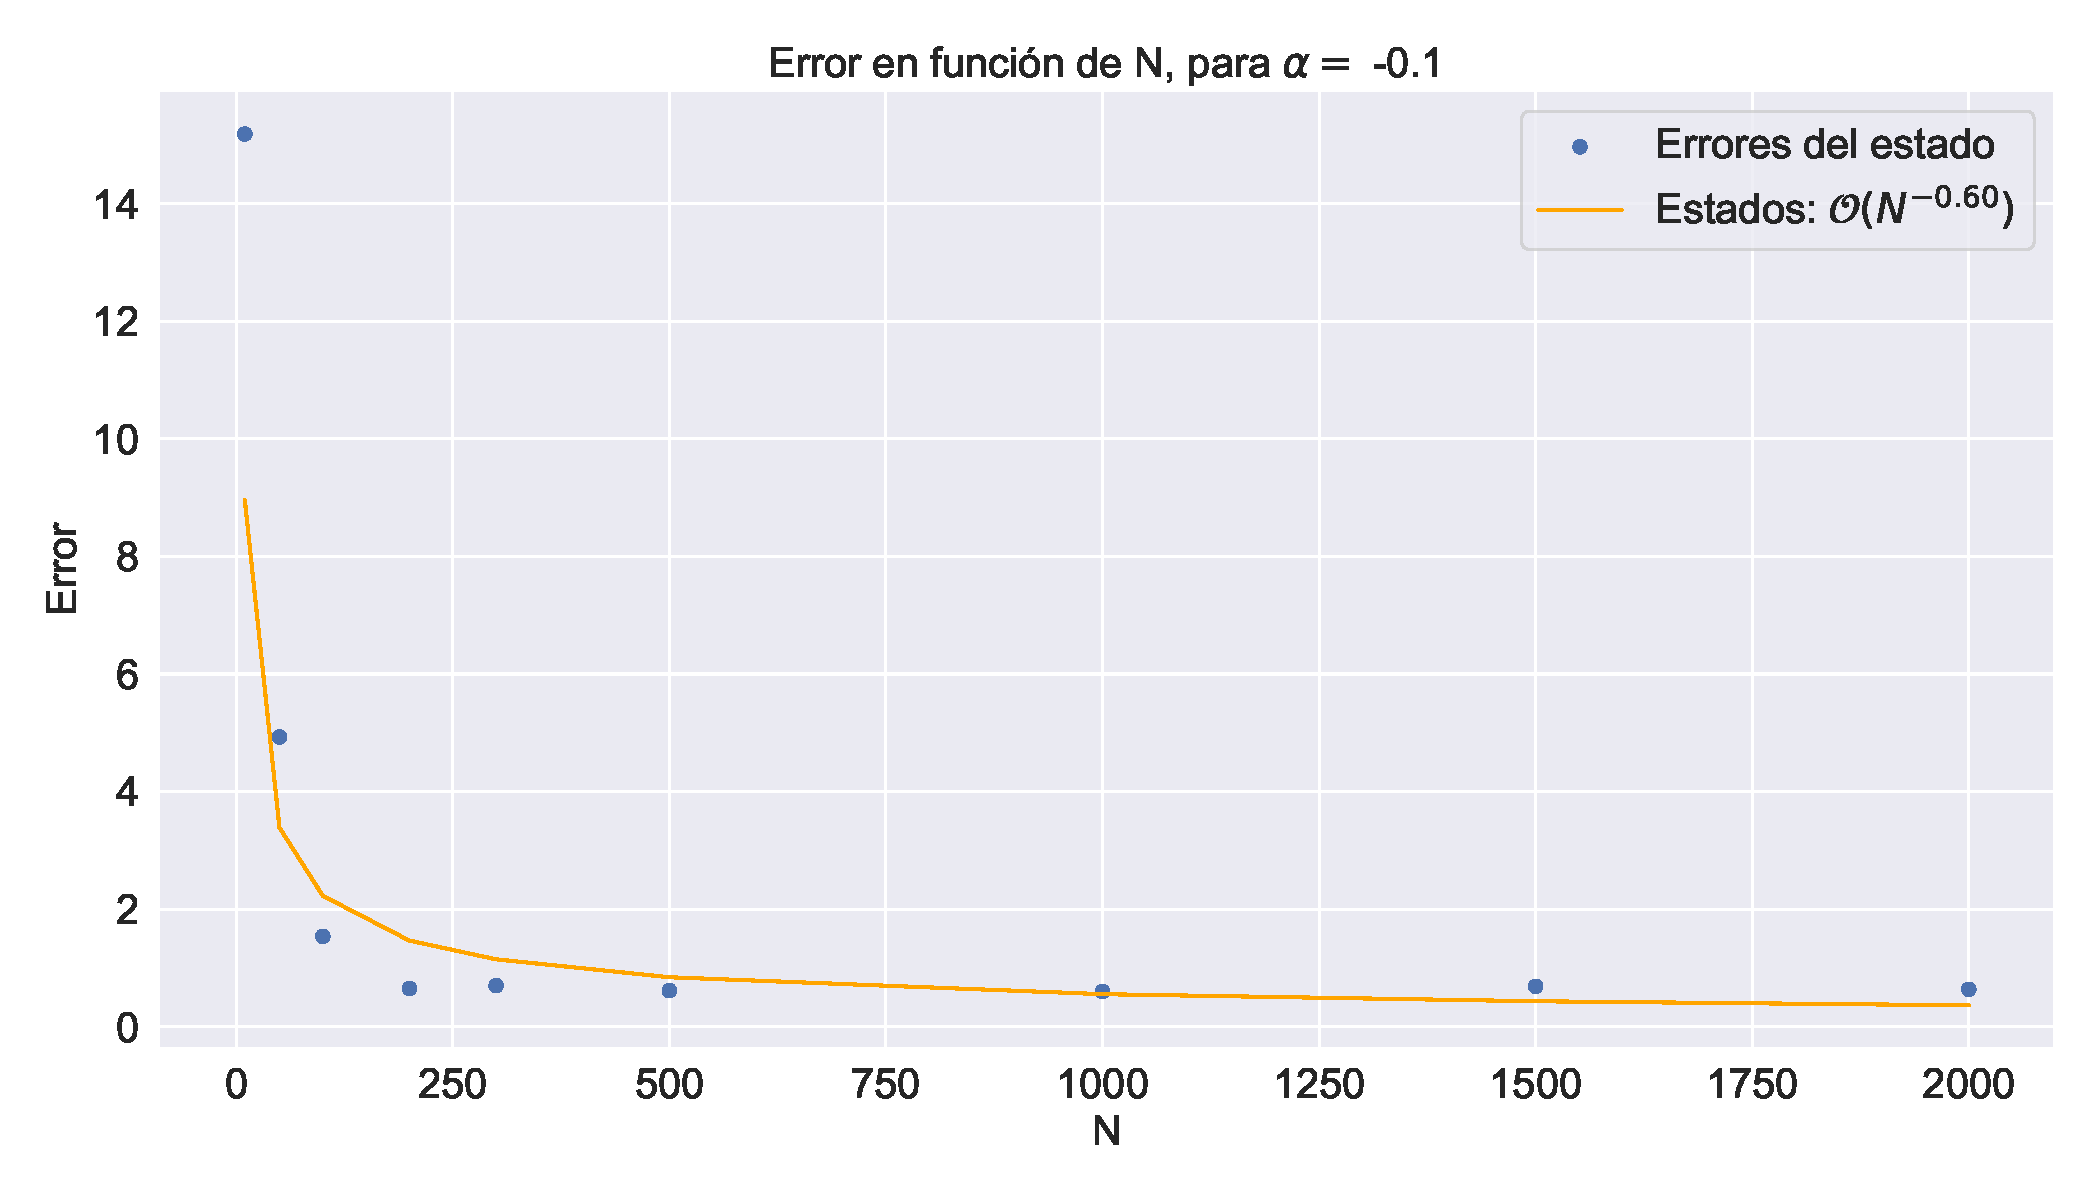
\includegraphics[width=\linewidth]{img/content/chapter4/linear_error_01.pdf}
    \caption{$\alpha = -0.1$}
    \label{fig:linear_error_01}
    \end{subfigure}
     \begin{subfigure}[b]{0.49\textwidth}
         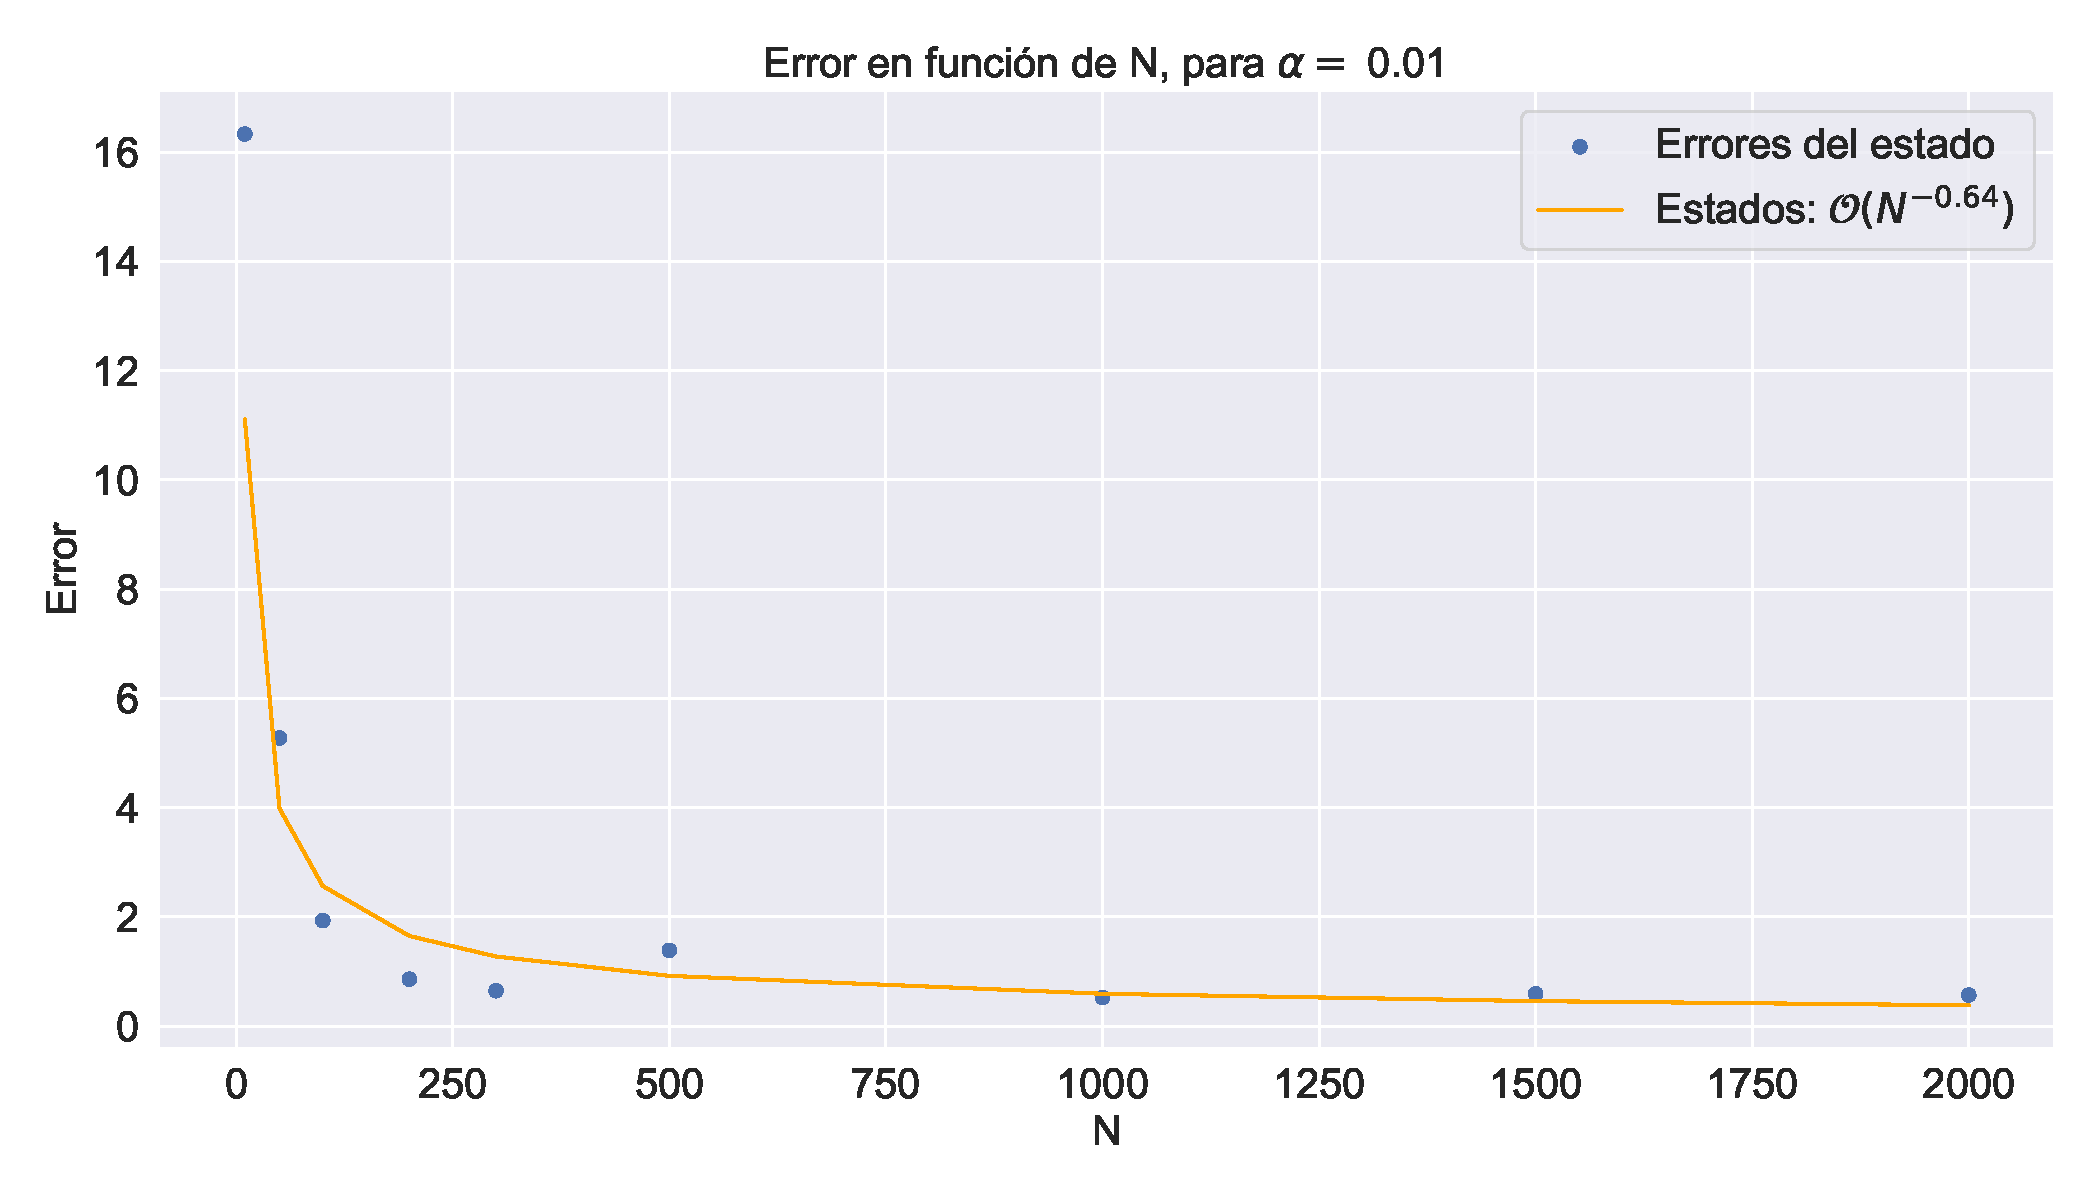
\includegraphics[width=\linewidth]{img/content/chapter4/linear_error_001.pdf}
    \caption{$\alpha = 0.01$}
    \label{fig:linear_error_001}
    \end{subfigure}
     \begin{subfigure}[b]{0.49\textwidth}
        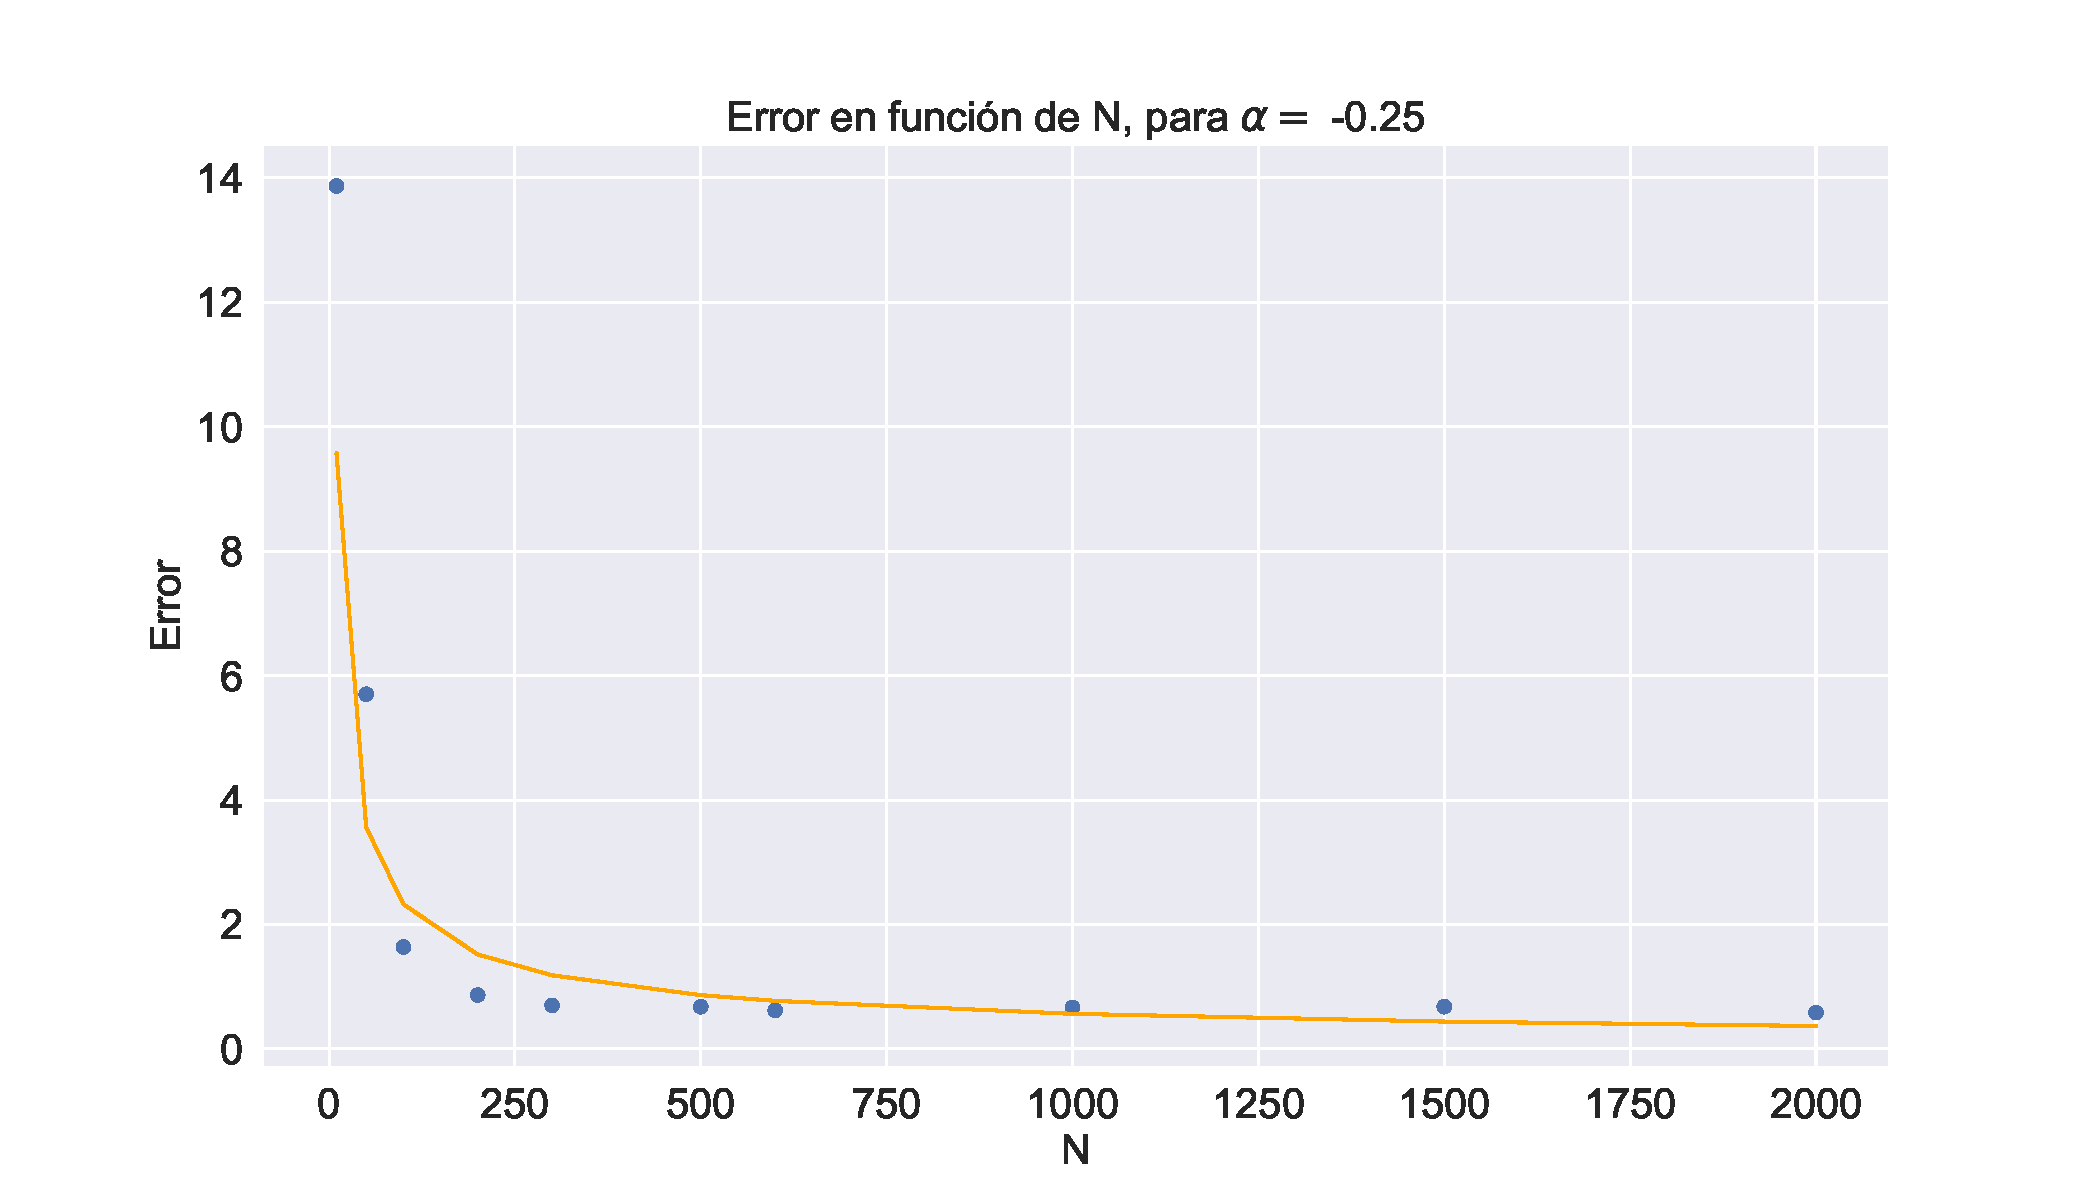
\includegraphics[width=\linewidth]{img/content/chapter4/linear_error_025.pdf}
    \caption{$\alpha = -0.25$}
    \label{fig:linear_error_025}
    \end{subfigure}    
    \caption{Error en norma para el estado en función de $N$ para distintos valores de $\alpha$.}
\end{figure}

\subsection{Comparación para modelos epidemiológicos con otros filtros}

Ahora se compara el filtro con otros filtros no lineales presentados en los preliminares, que vendrían siendo Extended Kalman Filter (EKF), Unscented Kalman Filter (UKF) y Particle Filters (PF), que, tal como se mencionó antes, son implementación propia para este trabajo. 

El sistema a considerar es el sistema SIR ya visto anteriormente
\begin{equation*}
    \begin{aligned}
    S_{k+1} &= S_k -\beta S_k I_k, \\
    I_{k+1} &= I_k + \beta S_k I_k - \gamma I_k, \\
    S_{k+1} &= R_k + \gamma I_k,
    \end{aligned}
\end{equation*}
en donde para esta subsección se considerarán $\beta$ y $\gamma$ conocidos y que la función de observación es
\begin{equation*}
    \mathbf{g}(S, I, R) = I,
\end{equation*}
es decir, solo se observan los infectados.

Se estudia primero el caso en que se prueban los filtros para $\beta = 1.0$ y $\gamma = 0.3$ y ruidos normales centrados con matrices de covarianza
\begin{equation*}
    \mathbf{Q} = \text{diag}(\sigma, \sigma, \sigma), \quad \mathbf{R} = \text{diag}(\sigma),
\end{equation*}
en donde $\sigma$ variará en cada experimento para poder visualizar cómo se comporta cada filtro en presencia de mayor ruido.

Se utiliza como condición inicial real $\mathbf{x}_0 = (0.9, 0.1, 0.0)$, prior para la condición inicial una variable aleatoria normal centrada en $\hat{\mathbf{x}}_0 = (0.9, 0.05, 0.05)$ con matriz de covarianza $\mathbf{Q}_0 = (0.01, 0.01, 0.01)$. Para el EKF se utilizan diferencias finitas centradas para la aproximación del Jacobiano de la dinámica con precisión $\varepsilon=10^{-6}$, para PF se utilizaron $N_p = 5000$ partículas y para KKF se utilizó $N=1000$ como dimensión de aproximación de los operadores. En las figuras \ref{fig:nonlinear_filters_sir_sigma_01}, \ref{fig:nonlinear_filters_sir_sigma_001} y \ref{fig:nonlinear_filters_sir_sigma_0001} se observan los resultados para $\sigma \in \{0.1, 0.01, 0.001\}$, seguido de las tablas \ref{tab:errores_sigma_01}, \ref{tab:errores_sigma_001} y \ref{tabla:errores_sigma_0001} que contienen el detalle de los errores para cada estado y cada filtro.

\begin{figure}[h!]
    \centering
    \begin{subfigure}[b]{0.49\textwidth}
        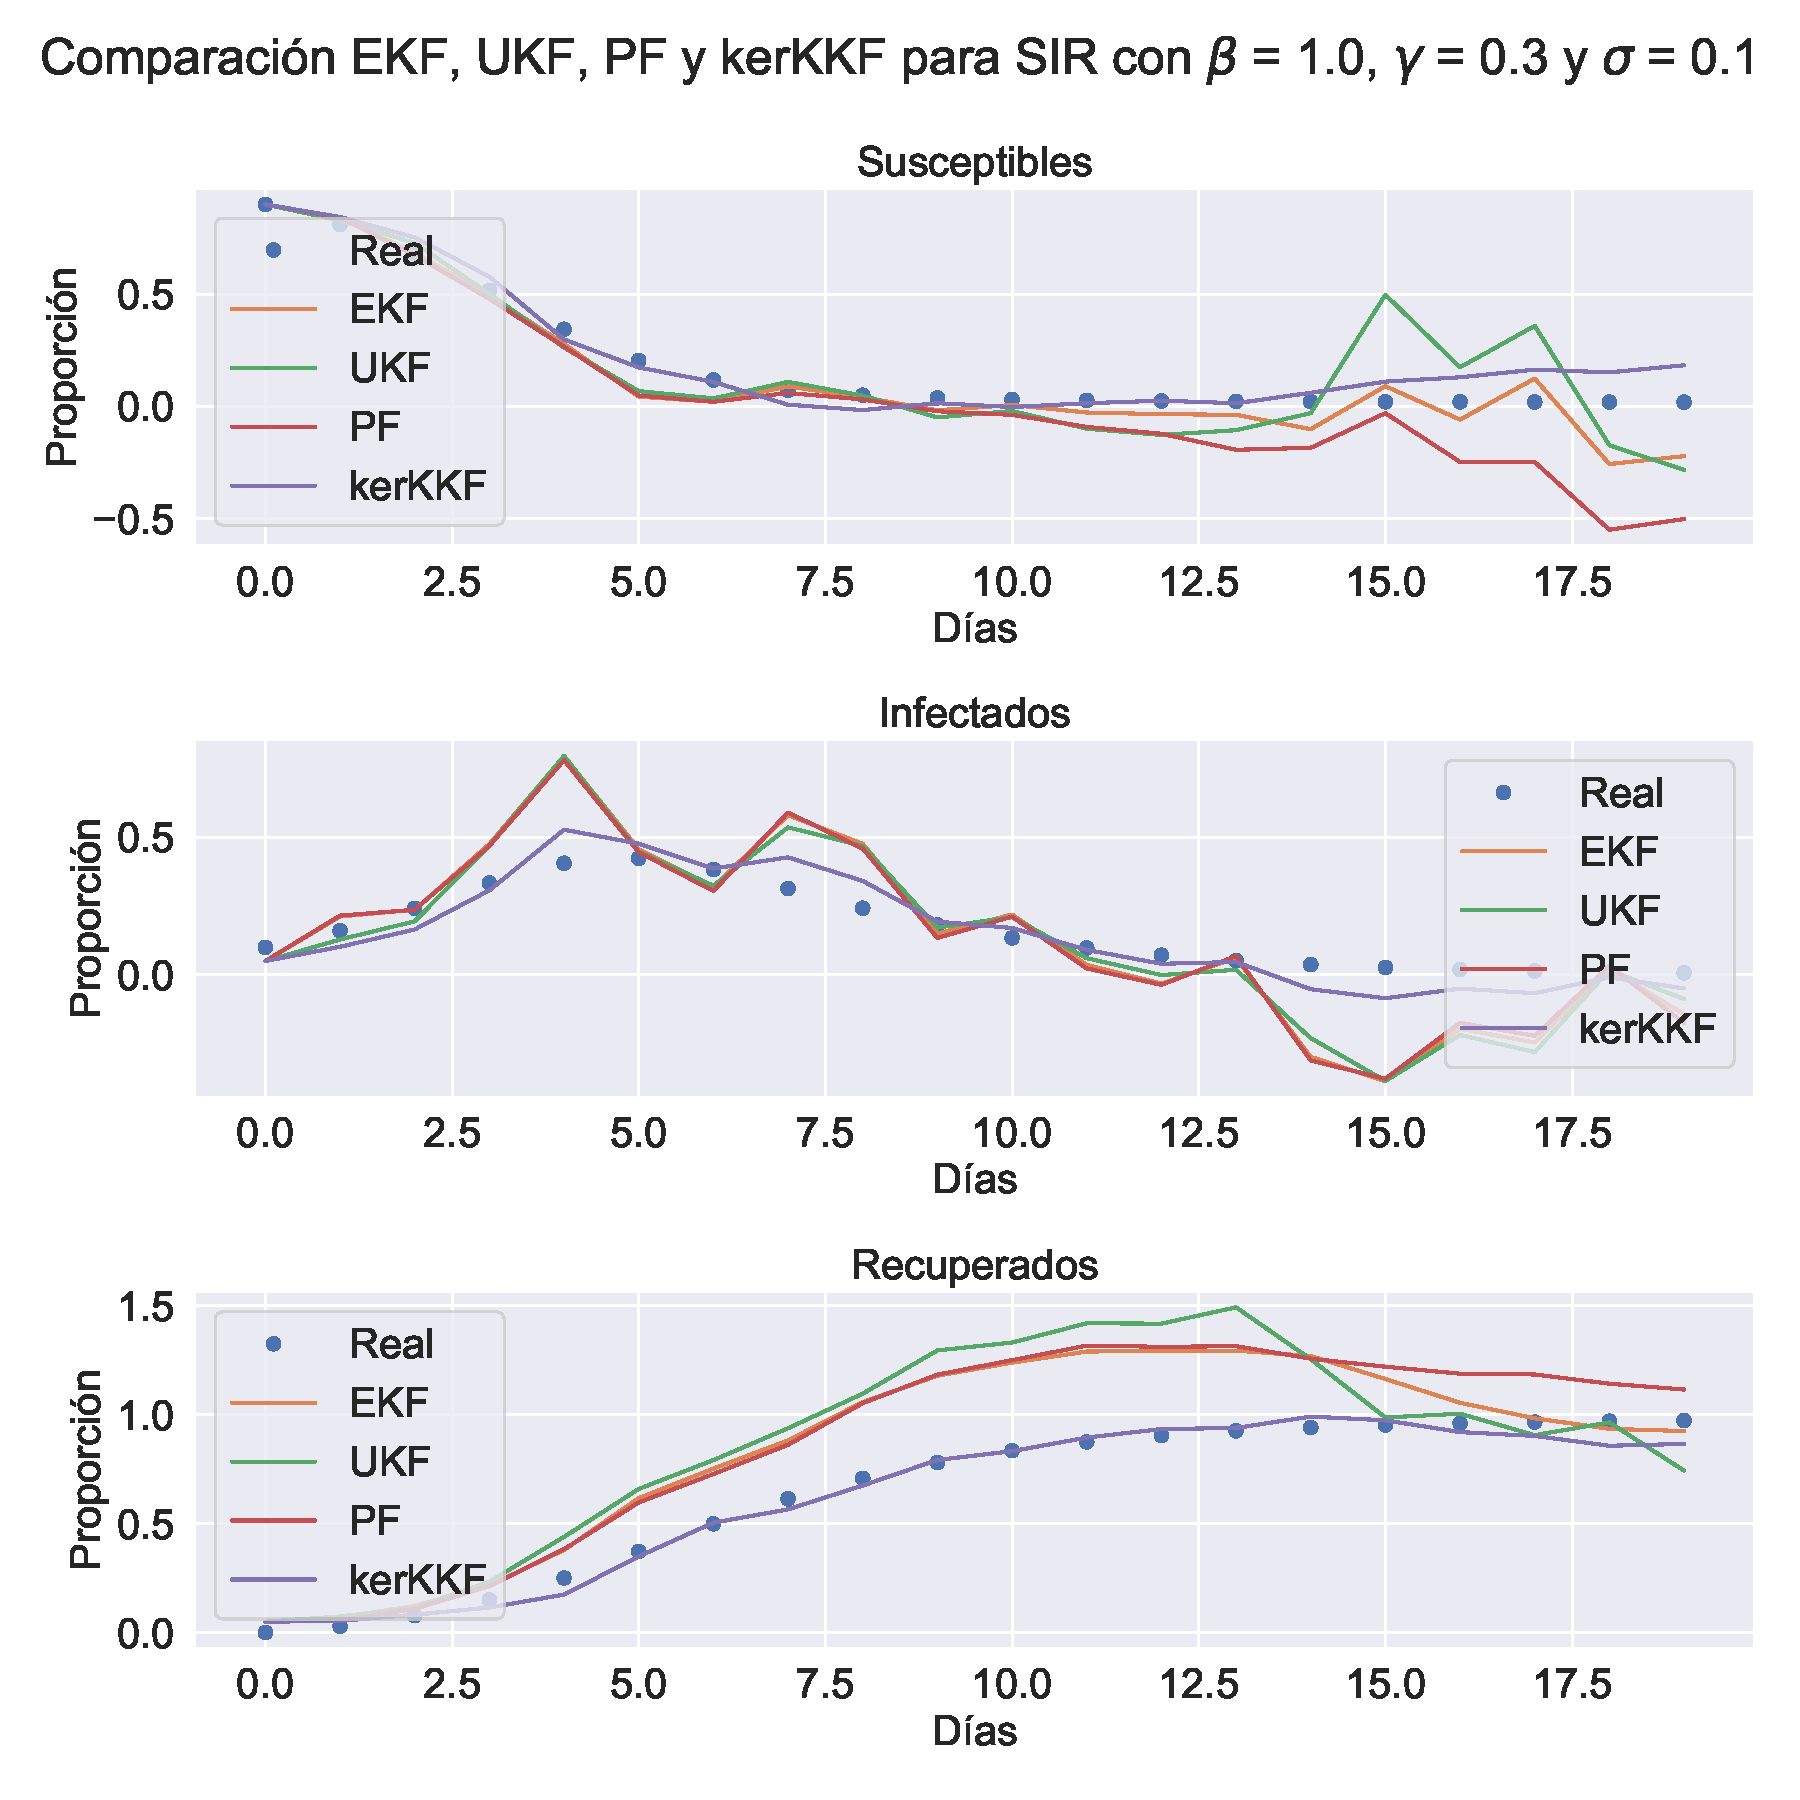
\includegraphics[width=0.9\linewidth]{img/content/chapter4/nonlinear_filters_sir_sigma_01.pdf}
    \caption{$\sigma = 0.1$.}
    \label{fig:nonlinear_filters_sir_sigma_01}
    \end{subfigure}
    \begin{subfigure}[b]{0.49\textwidth}
        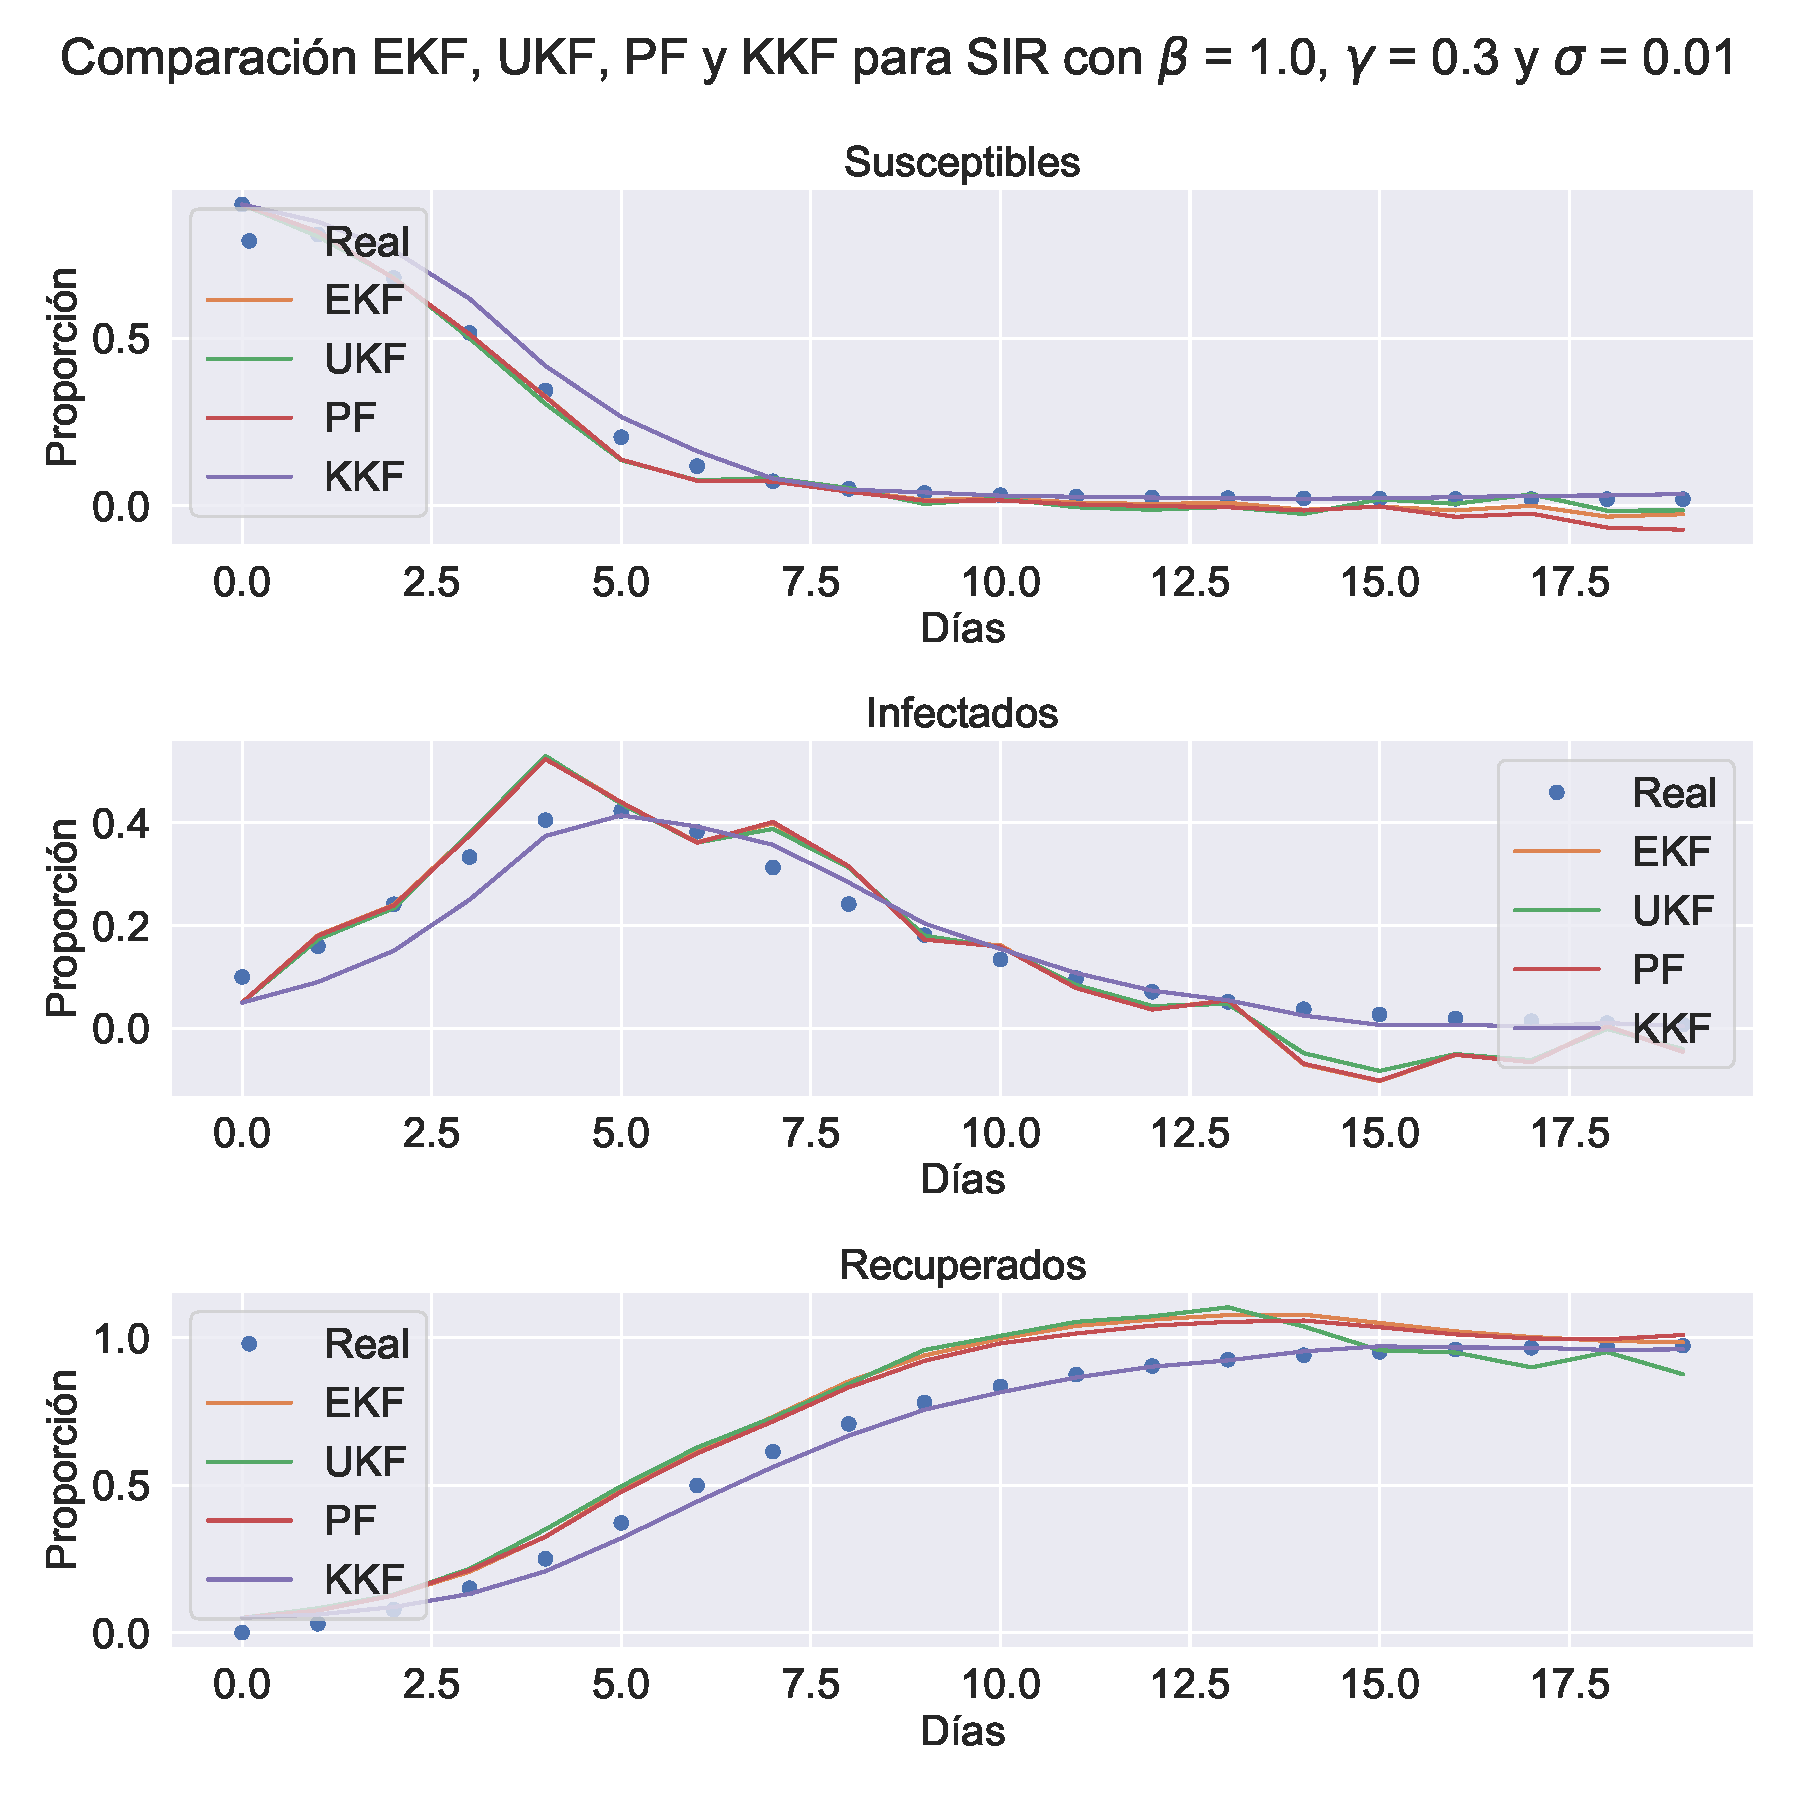
\includegraphics[width=0.9\linewidth]{img/content/chapter4/nonlinear_filters_sir_sigma_001.pdf}
    \caption{$\sigma = 0.01$.}
    \label{fig:nonlinear_filters_sir_sigma_001}
    \end{subfigure}
    \begin{subfigure}[b]{0.49\textwidth}
        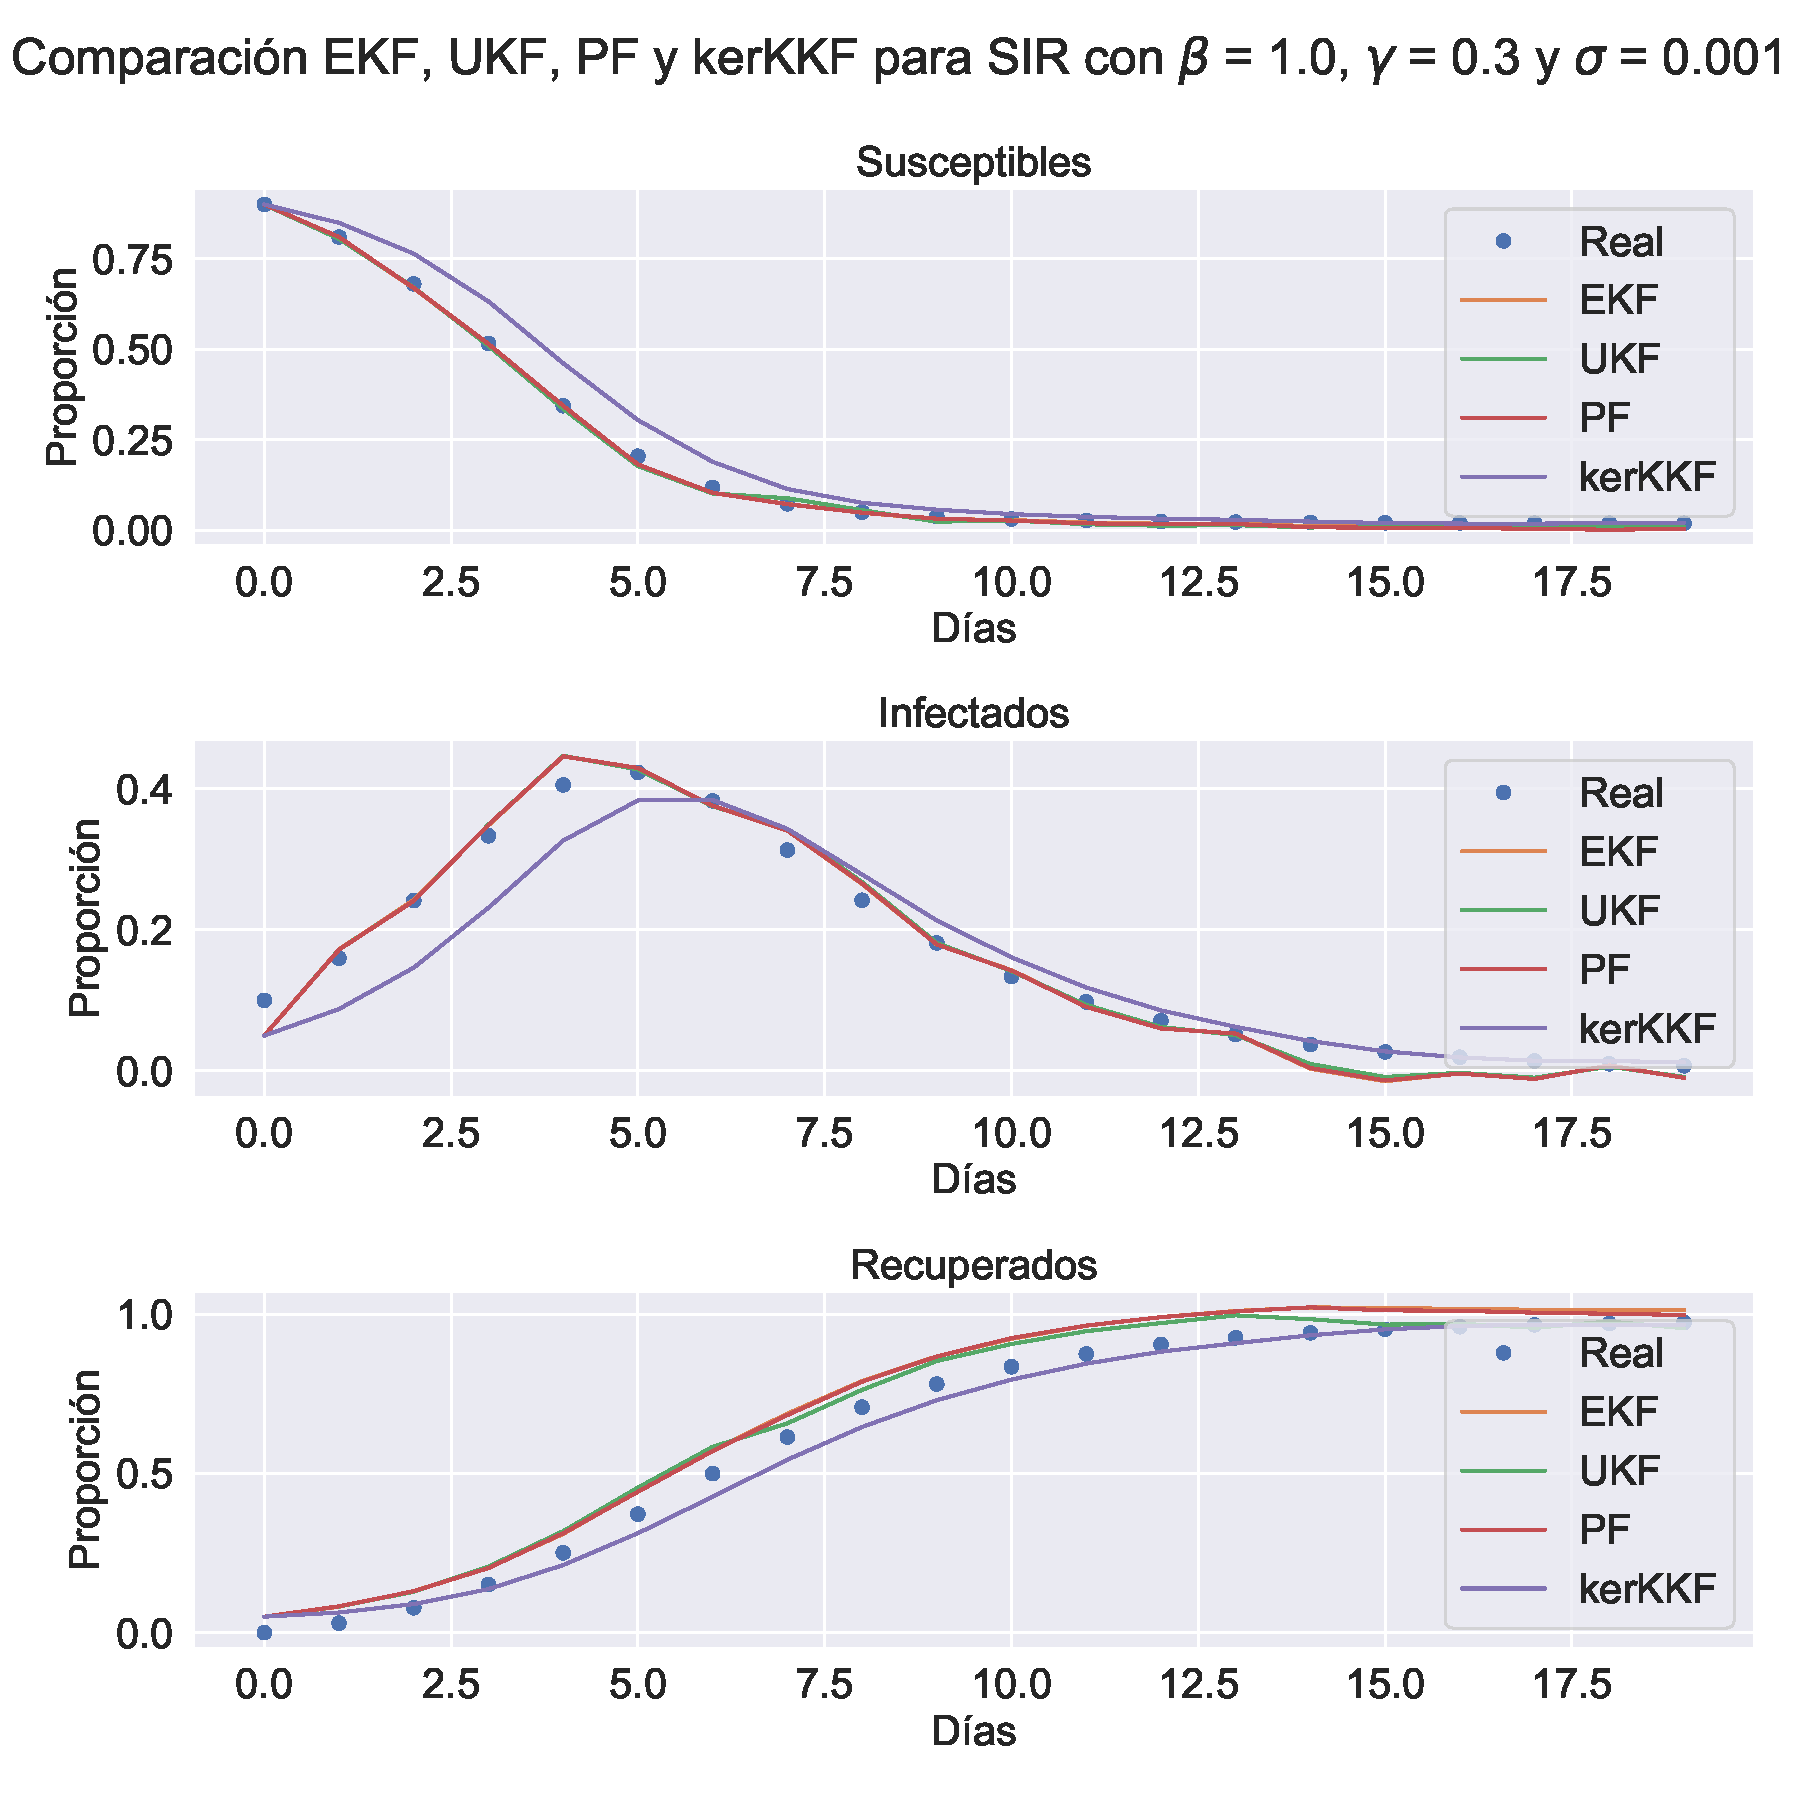
\includegraphics[width=0.9\linewidth]{img/content/chapter4/nonlinear_filters_sir_sigma_0001.pdf}
    \caption{$\sigma = 0.001$.}
    \label{fig:nonlinear_filters_sir_sigma_0001}
    \end{subfigure}
    \caption{Comparación de resultados de las trayectorias generadas por los filtros EKF (naranja), UKF (verde), PF (rojo) y KKF (púrpura), junto con la trayectoria real (puntos azules) sin ruidos, ni de dinámica ni de observación, esto para cada uno de los estados del modelo SIR. $\sigma$ es variable para (a), (b) y (c), mientras que $\beta = 1.0$ y $\gamma = 0.3$ fijos.}
\end{figure}

\begin{table}[h!]
    \caption{Errores de los distintos filtros con respecto a la trayectoria real, para distintos valores de la diagonal de la matriz de covarianza del ruido de dinámica $\sigma$.}
    \begin{subtable}{\linewidth}
        \centering
    \caption{$\sigma = 0.1$}
    \begin{tabular}{|c|c|c|c|c|}
    \hline
    \textbf{Estado} & \textbf{EKF} & \textbf{UKF} & \textbf{PF} & \textbf{KKF} \\ \hline
    S & 0.4757 & 0.7738 & 0.9571 & 0.3330 \\ \hline
    I & 0.8665 & 0.8300 & 0.8553 & 0.3015 \\ \hline
    R & 1.1360 & 1.4221 & 1.2151 & 0.2209 \\ \hline
    \end{tabular}
    \label{tab:errores_sigma_01}
    \end{subtable}
    \begin{subtable}{\linewidth}
        \centering
    \caption{$\sigma = 0.01$}
    \begin{tabular}{|c|c|c|c|c|}
    \hline
    \textbf{Estado} & \textbf{EKF} & \textbf{UKF} & \textbf{PF} & \textbf{KKF} \\ \hline
    S & 0.1277 & 0.1328 & 0.1783 & 0.1737 \\ \hline
    I & 0.2801 & 0.2565 & 0.2779 & 0.1709 \\ \hline
    R & 0.4881 & 0.5135 & 0.4337 & 0.1329 \\ \hline
    \end{tabular}
    \label{tab:errores_sigma_001}
    \end{subtable}
    \begin{subtable}{\linewidth}
        \centering
    \caption{$\sigma = 0.001$}
    \begin{tabular}{|c|c|c|c|c|}
    \hline
    \textbf{Estado} & \textbf{EKF} & \textbf{UKF} & \textbf{PF} & \textbf{KKF} \\ \hline
    S & 0.0417 & 0.0528 & 0.0493 & 0.2320 \\ \hline
    I & 0.1023 & 0.0985 & 0.1022 & 0.1996 \\ \hline
    R & 0.3070 & 0.2489 & 0.2983 & 0.1710 \\ \hline
    \end{tabular}
    \label{tabla:errores_sigma_0001}
    \end{subtable}
\end{table}

Se observa que KKF logra superar en error a todos los otros filtros con creces en el caso en que $\sigma \in \{ 0.1, 0.01\}$, aunque para el caso en donde hay menor ruido los resultados son bastante similares. Esto mostraría que el filtro tiene un mejor desempeño en comparación con los otros filtros en escenarios de mayor incertidumbre.

Se muestra ahora el caso en que $\sigma = 0.01$ fijo y varía el parámetro $\beta \in \{0.6, 0.9, 1.5\}$, en donde el objetivo es ver cómo cambian los resultados en función de $\beta$, que es en algún sentido el parámetro que cuantifica la no linealidad del sistema. Dado que $\gamma$ en realidad representa una relación lineal, se deja fijo en $\gamma = 0.3$. Se utilizan los mismos valores para todo el resto de configuraciones. Los resultados se pueden apreciar en las figuras \ref{fig:nonlinear_filters_sir_beta_06}, \ref{fig:nonlinear_filters_sir_beta_09} y \ref{fig:nonlinear_filters_sir_beta_15}, y en las tablas \ref{tab:errores_beta_gamma_06}, \ref{tab:errores_beta_gamma_09} y \ref{tab:errores_beta_gamma_15}.

Además, se midió el error en norma de los filtros para $50$ valores de $\beta$ entre $0.1$ y $2.5$ equiespaciados, manteniendo todo el resto de parámetros sin cambios. El resultado se puede observar en la figura \ref{fig:nonlinear_filters_sir_error_beta}, en donde KKF tiene un mejor desempeño a nivel general.

\subsection{Estimación de parámetros de modelos epidemiológicos}

A continuación se prueba la metodología para estimación de parámetros, que se compara con Markov Chain Monte Carlo, utilizando como \textit{samplers} Differential Evolution Metropolis (DEMetropolisZ) \cite{terBraak2008DifferentialChains}, que es un \textit{sampler} no basado en gradiente, y No-U-Turn Sampler (NUTS) \cite{Hoffman2014TheCarlo}, que está basado en gradiente y además es de los más utilizados cuando hay un sistema dinámico subyacente implementado en PyMC \cite{Patil2010PyMC:Python}.

Para DEMetropolisZ se utilizarán 20000 iteraciones de \textit{warm up}, es decir, no se utilizarán para la estimación y 20000 para estimación como tal. Mientras que para NUTS se utilizaron 150 y 150, respectivamente. Para la aproximación de Koopman, en los tres sistemas donde se probó, se utilizará $N=100$. Se realizaron 300 iteraciones del algoritmo \ref{alg:ParamEstim}, de las cuales la primera mitad se tomó como \textit{warm up} y la segunda mitad se considerará para la estimación. Para los 3 algoritmos, se hará el mismo procedimiento 8 veces en paralelo.

Se prueba la metodología de estimación de parámetros para el modelo SIR \eqref{eq:SIR}, esto es, lograr una estimación para $\beta$ y $\gamma$ en base a observaciones, tal como se encuentra en el algoritmo \ref{alg:ParamEstim}. Por lo que se considera el modelo con estados aumentados, que es

\begin{equation*}
    \begin{aligned}
        S_{k+1} &= S_k - \beta_k S_k I_k + \mathbf{w}_k^1 \\
        I_{k+1} &= I_k + \beta_k S_k I_k - \gamma_k I_k + \mathbf{w}_k^2 \\
        R_{k+1} &= R_k + \gamma_k I_k + \mathbf{w}_k^3 \\
        \beta_{k+1} &= \beta_k + \mathbf{w}_k^4 \\
        \gamma_{k+1} &= \gamma_k + \mathbf{w}_k^5
    \end{aligned}
\end{equation*}

Se utilizan como parámetros reales $\beta=1.3$ y $\gamma=0.5$, se utiliza como condición inicial para el estado aumentado $\mathbf{x}_0 = (0.9, 0.1, 0.0, 1.3, 0.5)$, y se entrega también como media del prior de la condición inicial $\hat{\mathbf{x}}_0 = (0.9, 0.1, 0.0, 0.1, 0.1)$, con matriz de covarianza inicial
\begin{equation*}
    \mathbf{Q}_0 = \text{diag}(0.001, 0.001, 0.001, 1, 1).
\end{equation*}

Es decir, se entrega como condición inicial para los parámetros $0.1$ y se espera que el algoritmo converja a los parámetros reales. Se considera que los estados observables son $S$ e $I$, es decir
\begin{equation*}
    \mathbf{g}(S, I, R, \beta, \gamma) = (S, I)
\end{equation*}
y se consideran ruidos normales aditivos, centrados y con matrices de covarianza, para la dinámica y la observación, respectivamente
\begin{equation*}
    \mathbf{Q} = \text{diag}(0.001, 0.001, 0.001, 1, 1), \quad \mathbf{R} = \text{diag}(0.001, 0.001).
\end{equation*}

Se simula el sistema a $20$ unidades de tiempo y para muestrear puntos desde el estado se utiliza una variable aleatoria cuyas primeras tres entradas vienen desde una Dirichlet de parámetro $(1,1,1)$ y las otras dos desde Uniformes en $[0.5, 1.5]$ y $[0.1, 0.5]$, respectivamente. 

Se realizan $300$ iteraciones para el procedimiento expuesto en el algoritmo \ref{alg:ParamEstim}. Este procedimiento se hace $8$ veces en paralelo, por lo que hay $8$ filtros, que se denotarán cadenas, que están estimando el parámetro en paralelo. 

En la figura \ref{fig:param_estim_SIR} se muestra el resultado del filtro en la última iteración y la evolución del parámetro estimado en función de las iteraciones, todo esto solo para la primera cadena de manera ilustrativa. En la figura \ref{fig:density_param_estim_SIR} se muestran las densidades de probabilidad generadas por cada cadena, comparadas con el valor real del parámetro. Si estas se promedian, queda una densidad de probabilidad que es mucho más robusta para la estimación del parámetro, resultado que se puede observar en la figura \ref{fig:mean_density_param_estim_SIR}.



\begin{figure}[h!]
    \centering
    \begin{subfigure}[b]{0.8\textwidth}
        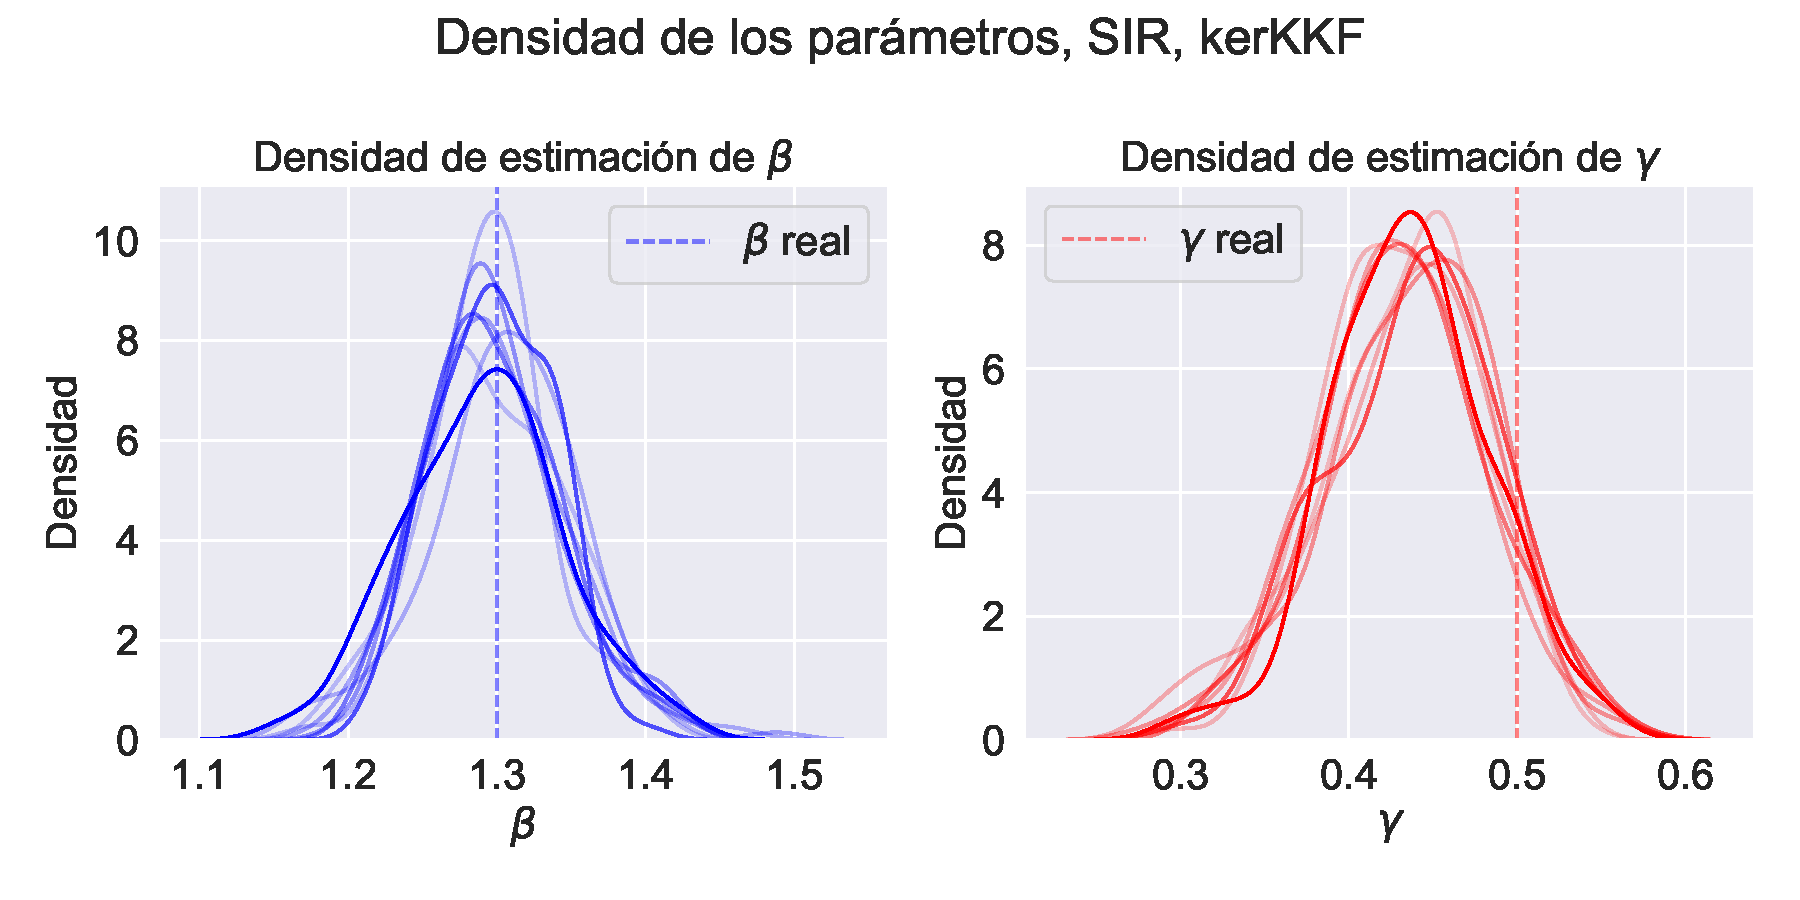
\includegraphics[width=\linewidth]{img/content/chapter4/nonlinear_filters_sir_params_density.pdf}
        \caption{}
        \label{fig:density_param_estim_SIR}
    \end{subfigure}
    \begin{subfigure}[b]{0.8\textwidth}
        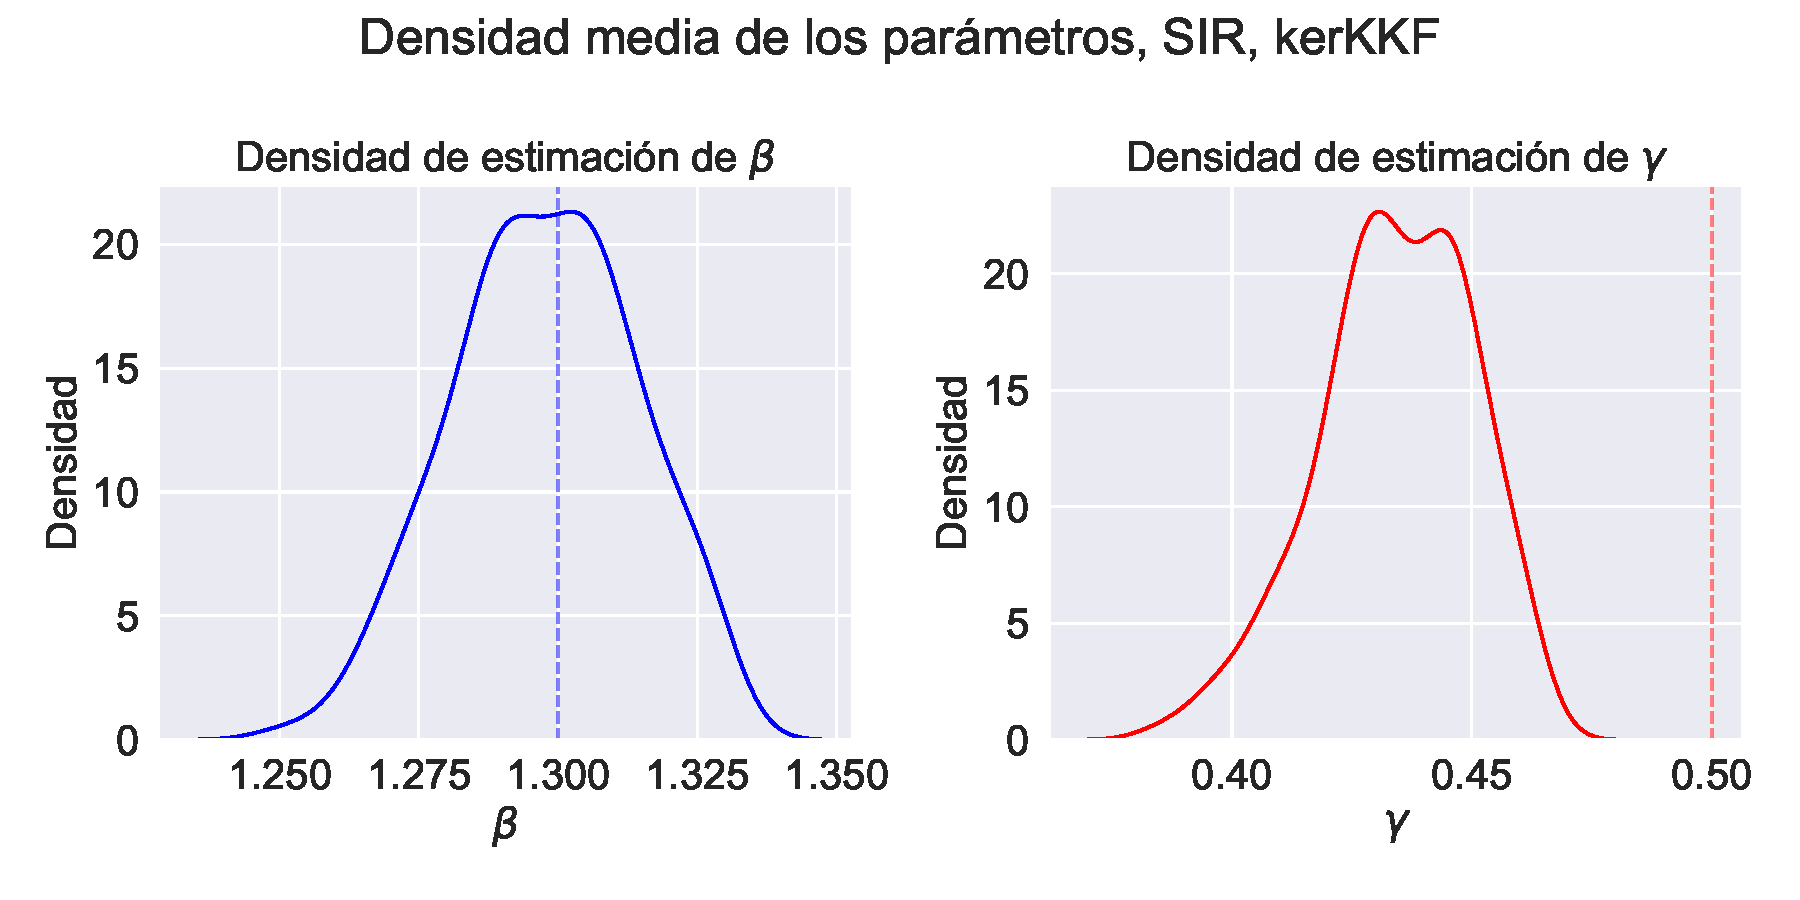
\includegraphics[width=\linewidth]{img/content/chapter4/nonlinear_filters_sir_params_density_mean.pdf}
        \caption{}
        \label{fig:mean_density_param_estim_SIR}
    \end{subfigure}
    \caption{A la izquierda el resultado para $\beta$ y a la derecha para $\gamma$, parámetros del modelo SIR \eqref{eq:SIR}. En línea punteada vertical se encuentra el valor real del parámetro. \\
    (a) Densidades de probabilidad creadas por cada cadena solo considerando las iteraciones posteriores al \textit{warm up}. Por cada una son $8$ densidades correspondientes a cada cadena. \\
    (b) Densidades de probabilidad resultante de promediar las $8$ densidades creadas por cada cadena.}
    
\end{figure}

Se repite el mismo procedimiento con el modelo SIRS para estimar sus parámetros $\alpha$, $\beta$ y $\gamma$, que con el estado aumentado queda
\begin{equation*}
    \begin{aligned}
        S_{k+1} &= S_k - \beta_k S_k I_k + \alpha_k R_k + \mathbf{w}_k^1 \\
        I_{k+1} &= I_k + \beta_k S_k I_k - \gamma_k I_k + \mathbf{w}_k^2 \\
        R_{k+1} &= R_k + \gamma_k I_k - \alpha_k R_k + \mathbf{w}_k^3 \\
        \alpha_{k+1} &= \alpha_k + \mathbf{w}_k^4 \\
        \beta_{k+1} &= \beta_k + \mathbf{w}_k^5 \\
        \gamma_{k+1} &= \gamma_k + \mathbf{w}_k^6.
    \end{aligned}
\end{equation*}

Para el experimento se utilizaron como valores reales reales $\alpha = 0.2$, $\beta = 1.4$, $\gamma = 0.4$ y condición inicial para el resto de estados $(S_0, I_0, R_0) = (0.9, 0.1, 0.0)$. Se entrega como prior para la condición inicial una normal centrada en $\hat{\mathbf{x}}_k = (0.9, 0.1, 0.0, 0.1, 0.1, 0.1)$ con matriz de covarianza
\[
\mathbf{Q}_0 = \text{diag}(0.01, 0.01, 0.01, 10, 10, 10).
\]

Como función de observación ahora se considera que únicamente es posible observar a los infectados, es decir
\[
\mathbf{g}(S, I, R, \alpha, \beta, \gamma) = I,
\]
por lo que se tiene menos información incluso para este caso que para el anterior, en que se deseaba estimar menos parámetros.

Como distribuciones asociadas a la dinámica y la observación se utiliza un ruido normal aditivo, centrado y con matriz de covarianza y varianza, respectivamente
\[
\mathbf{Q} = \text{diag}(0.001, 0.001, 0.001, 10, 10, 10), \quad \mathbf{R} = 0.01
\]
dado que para la observación es necesaria una variable univariada.

Para muestrear desde el estado se utiliza una variable aleatoria cuyas primeras tres entradas provienen de una Dirichlet de parámetro $(1,1,1)$ y las otras tres de variables aleatorias uniformes en $[0.1, 1.0]$, $[0.1, 0.5]$ y $[0.1, 0.5]$, respectivamente. Se simula el sistema a $20$ unidades temporales.

En la figura \ref{fig:nonlinear_filters_sirs_params} se observa la solución de KKF para el sistema, esto para la última iteración del algoritmo \ref{alg:ParamEstim} y en la primera cadena de las $8$ muestreadas, mientras que en la figura \ref{fig:nonlinear_filters_sirs_params_evolution} se puede ver la evolución del parámetro a través de las iteraciones, esto también para la primera cadena.

Análogo a lo hecho antes, se puede convertir la evolución del parámetro a través de las iteraciones del algoritmo en una densidad de probabilidad, para la cual se consideran solo la segunda mitad de las iteraciones, dejando la primera mitad como \textit{warm up}. Esto se puede ver en la figura \ref{fig:nonlinear_filters_sirs_params_density}, en donde se dejan las $8$ cadenas y en la figura \ref{fig:nonlinear_filters_sirs_params_density_mean} la cadena media para cada uno de los parámetros.

El algoritmo logra acercarse mucho a los parámetros reales de cada sistema, dejando al menos el parámetro real en su intervalo de confianza de nivel $95$\%.

Por último, se prueba para el modelo SEIR, que tiene 4 estados y 4 parámetros por estimar, $\alpha$, $\beta$, $\gamma$ y $\delta$.
\begin{equation*}
    \begin{aligned}
        S_{k+1} &= S_k - \beta_k S_k I_k + \alpha_k R_k + \mathbf{w}_k^1 \\
        E_{k+1} &= E_k + \beta_k S_k I_k - \delta_k E_k + \mathbf{w}_k^2 \\
        I_{k+1} &= I_k + \delta_k E_k - \gamma_k I_k + \mathbf{w}_k^3 \\
        R_{k+1} &= R_k + \gamma_k I_k - \alpha_k R_k + \mathbf{w}_k^4 \\
        \alpha_{k+1} &= \alpha_k + \mathbf{w}_k^5 \\
        \beta_{k+1} &= \beta_k + \mathbf{w}_k^6 \\
        \gamma_{k+1} &= \gamma_k + \mathbf{w}_k^7 \\
        \delta_{k+1} &= \delta_k + \mathbf{w}_k^8.
    \end{aligned}
\end{equation*}
Se simula el sistema a $20$ unidades de tiempo suponiendo que solo se observan los susceptibles y los infectados, es decir,
\begin{equation*}
    g(S, E, I, R, \alpha, \beta, \gamma, \delta) = (S, I).
\end{equation*}

Se puede ver en las figuras \ref{fig:nonlinear_filters_seir_params_density} y \ref{fig:nonlinear_filters_seir_params_density_mean} las densidades de probabilidad que se generan al estimar parámetros. Para poder estudiar el error en las trayectorias, se \textit{samplean} 30 muestras de parámetros desde las densidades de probabilidad generadas, con lo que se obtiene error promedio, desviación estándar para el error, error mínimo y error máximo, esto para cada modelo y cada método, lo que se puede observar en las tablas \ref{tab:metricas_traj_SIR}, \ref{tab:metricas_traj_SIRS} y \ref{tab:metricas_traj_SEIR}, mientras que las trayectorias \textit{sampleadas} se pueden encontrar en las figuras \ref{fig:SIR_traj_params}, \ref{fig:SIRS_traj_params} y \ref{fig:SEIR_traj_params}.

Se observa el rendimiento de los 3 algoritmos, para los 3 sistemas, es bastante similar, solo que KKF entrega intervalos de confianza más pequeños. El aspecto más relevante, por lejos, es el hecho de que KKF es mucho más rápido que DEMetropolisZ y NUTS, siendo incluso casi 10 veces más rápido que NUTS para el modelo SEIR. Esto es un aspecto relevante a considerar dado que NUTS, muy utilizado en muchas aplicaciones de modelos epidemiológicos para estimar parámetros, usualmente demora horas para poder ejecutarse y debe llevarse a supercomputadores. Puede que esta nueva metodología sea más eficiente en este sentido y logre aligerar tareas de computo muy tediosas y disminuir las horas de espera.

\begin{table}[h!]
    \centering
    \caption{Estimación de parámetros del modelo SIR (IC 95\%).} 
    \begin{tabular}{|c|c|c|c|c|}
    \hline
    \textbf{Parámetro} & \textbf{Real} & \textbf{DEMetropolisZ} & \textbf{NUTS} & \textbf{KKF}  \\ \hline
    $\beta$ & 1.3 & 1.59 (0.96, 2.22) & 1.33 (1.31, 1.35) & 1.39 (1.35, 1.42) \\ \hline
    $\gamma$ & 0.5 & 0.69 (0.23, 1.16) & 0.45 (0.44, 0.46) & 0.47 (0.45, 0.49) \\ \hline
    \end{tabular}
    \label{tab:SIR_params}
\end{table}

\begin{table}[h!]
    \centering
    \caption{Estimación de parámetros del modelo SIRS (IC 95\%).} 
    \begin{tabular}{|c|c|c|c|c|}
    \hline
    \textbf{Parámetro}& \textbf{Real} & \textbf{DEMetropolisZ} & \textbf{NUTS} & \textbf{KKF}  \\ \hline
    $\alpha$ & 0.2 & 0.31 (-0.25, 0.88) & 0.17 (0.16, 0.18) & 0.19 (0.17, 0.21) \\ \hline
    $\beta$ & 1.3 & 1.4 (0.88, 1.92) & 1.34 (1.31, 1.36) & 1.3 (1.24, 1.36) \\ \hline
    $\gamma$ & 0.5 & 0.57 (0.22, 0.93) & 0.51 (0.50, 0.52) & 0.44 (0.40, 0.48) \\ \hline
    \end{tabular}
    \label{tab:SIRS_params}
\end{table}

\begin{table}[h!]
    \centering
    \caption{Estimación de parámetros del modelo SEIR (IC 95\%).} 
    \begin{tabular}{|c|c|c|c|c|}
    \hline
    \textbf{Parámetro}& \textbf{Real} & \textbf{DEMetropolisZ} & \textbf{NUTS} & \textbf{KKF}  \\ \hline
    $\alpha$ & 0.2 & 0.92 (0.54, 1.31) & 0.15 (0.13, 0.16) & 0.09 (0.08, 0.10) \\ \hline
    $\beta$ & 1.3 & 2.0 (1.96, 2.03) & 1.27 (1.2, 1.35) & 0.99 (0.95, 1.03) \\  \hline
    $\gamma$ & 0.4 & 0.55 (0.44, 0.66) & 0.47 (0.44, 0.51)
 & 0.37 (0.36, 0.38)\\ \hline
    $\delta$ & 0.5 & 0.37 (0.25, 0.50) & 0.39 (0.37, 0.40) & 0.64 (0.62, 0.66)\\ \hline
    \end{tabular}
    \label{tab:SEIR_params}
\end{table}

\begin{table}[h!]
    \centering
    \begin{tabular}{|c|c|c|c|}
    \hline
    \textbf{Métrica} & \textbf{DEMetropolisZ} & \textbf{NUTS} & \textbf{KKF} \\
    \hline
    Error promedio & 0.730 & 0.170 & 0.190 \\
    \hline
Desviación estándar & 0.369 & 0.015 & 0.023 \\
    \hline
Error mínimo & 0.212 & 0.137 & 0.156 \\
    \hline
Error máximo & 2.029 & 0.203 & 0.240 \\
    \hline
    \end{tabular}
    \caption{Métricas para trayectorias \textit{sampleadas} del modelo SIR.}
    \label{tab:metricas_traj_SIR}
\end{table}

\begin{table}[h!]
    \centering
    \begin{tabular}{|c|c|c|c|}
\hline
\textbf{Métrica} & \textbf{DEMetropolisZ} & \textbf{NUTS} & \textbf{KKF} \\
\hline
Error promedio & 1.150 & 0.160 & 0.260 \\
\hline
Desviación estándar & 0.654 & 0.015 & 0.110 \\
\hline
Error mínimo & 0.450 & 0.131 & 0.030 \\
\hline
Error máximo & 3.590 & 0.192 & 0.511 \\
\hline
\end{tabular}
    \caption{Métricas para trayectorias \textit{sampleadas} del modelo SIRS.}
    \label{tab:metricas_traj_SIRS}
\end{table}

\begin{table}[h!]
    \centering
    \begin{tabular}{|c|c|c|c|}
\hline
\textbf{Métrica} & \textbf{DEMetropolisZ} & \textbf{NUTS} & \textbf{KKF} \\
\hline
Error promedio & 1.120 & 0.190 & 0.240 \\
\hline
Desviación estándar & 0.280 & 0.079 & 0.013 \\
\hline
Error mínimo & 0.612 & 0.082 & 0.215 \\
\hline
Error máximo & 1.749 & 0.464 & 0.269 \\
\hline
\end{tabular}
    \caption{Métricas para trayectorias \textit{sampleadas} del modelo SEIR.}
    \label{tab:metricas_traj_SEIR}
\end{table}

\begin{table}[h!]
    \centering
    \caption{Tiempos de ejecución para los distintos métodos y modelos, para estimación de parámetros, en segundos.} 
    \begin{tabular}{|c|c|c|c|}
    \hline
    \textbf{Modelo} & \textbf{DEMetropolisZ} & \textbf{NUTS} & \textbf{KKF}  \\ \hline
    \textbf{SIR} & 104.1 & 112.00 & 28.3 \\ \hline
    \textbf{SIRS} & 120.6 & 237.7 & 31.5 \\ \hline
    \textbf{SEIR} & 127.8 & 508.6 & 73.6 \\ \hline
    \end{tabular}
    \label{tab:ex_times}
\end{table}